%!TEX root = first try.tex

% \chapter{Background research for Criterion on Lateral Dynamics of Railway Bridges in Eurocode 1991-2}

% Eurocode is made by committees consist of experts from a variety of engineering fields. During the creating of Eurocode, it is believed that committee member will refer to existing scientific research to base code contents on. Since there isn't any explanation nor description for 1.2Hz criterion, this chapter aims to discover the supporting research behind this criterion. 

% Quoting mr. Paul Vos, one of the committee member composing Eurocode 1991-2 who is also a committee member of UIC ERRI D181 research committee, said a majority of the criteria/requirements regarding railway infrastructures are extracted from researching fruits of UIC. UIC stands for International Union of Railways. It regulates railway vehicle, infrastructure and maintenance standard for member countries all over the world. My investigation starts from reports created by ERRI, a scientific research department under UIC.

% \section{ERRI reports investigation}
% ERRI reports are created by ERRI committees, which are categorized into research topics. For example, committee D181, investigated lateral forces that acting on railway bridges. Among reports created by D181, origin of 1.2Hz criterion is found in RP6. 

% \subsection{Supporting report D181 RP6}\label{sec:1.2hz}

% Evidence of \cite{d181} is the origin of \cite[A.2.4.4.2.4(3)]{EC12} is found in \cite[p4.2: Lateral Frequencies]{d181}:

% In order to avoid the phenomena of lateral resonance in vehicles, the first natural frequency of lateral vibration of the span $f_{lt}$ such that:

% \begin{equation}
% f_{lt} \geq 1.2Hz
% \end{equation}

% The statement exactly coincides with criterion A.2.4.4.2.4(3) in Eurocode 1991. It is sufficient to acknowledge D181 RP6 as the origin of criterion A.2.4.4.2.4(3) because this report is created by UIC.

% The value of frequency limit, 1.2Hz is explained in \cite[p3.2: Criterion 2]{d181}:

% \begin{quote}
% To avoid the occurrence of resonance in the lateral motion of the vehicles due to the lateral motion of the bridge, a limit value lower than the first natural frequency $f_1t$ of the lateral vibration of the span studied should be fixed. The natural frequency for lateral movements is between 0.5 and 0.7 Hz for coaches and between 0.7 and 1 Hz for locomotives. We therefore propose a safety margin $F_{lt} \geq 1.2Hz$
% \end{quote}

% Till now, the origin of vehicle data involved in above explanation remains unknown. Since UIC publishes train vehicle standards to all its members including European Union, it is reasonable to believe researcher of Committee D181 use internal information of UIC to get the frequency of lateral vehicle moving.

% From this statement we can conclude that the background of 1.2Hz criterion is Eurocode 1991-2 avoids bridges having a first lateral natural frequency that falls between lateral vibrating frequency of running train. But this criterion can be judged as too conservative since it covers a frequency bandwidth of 0-1.2Hz, which is over 100\% exceeding the train frequency bandwidth 0.5-1.0Hz.

% It can also be concluded that the bridge is actually meeting the origin purpose of the criterion if the first lateral frequency of the bridge is out of the domain of train frequency. But it arouses another problem that trains' lateral movement frequency is completely dependent on train parameters. However, the train frequency domain proposed in RP6 is extracted from data obtained before 1996 in France. It means that for example, the train vehicle running on railways nowadays can be completely different from the train running before 1996. So updating train dynamics data is also essential to make use of this requirement.

% It's also important to study how did D181 committee obtained the train frequency data. The procedure is described in report D181 DT329 E\cite{d181dt329}. 

% \subsection{Supporting report D181 DT329 E}

% \subsubsection{Methodology adopted in D181 DT329 E}
% The methodology used to obtain train frequency was described as following quoting \cite[p.4]{d181dt329}:

% \begin{quote}
% The dynamic lateral response to the passage of different train types of various theoretical bridge models to be examined using VAMPIRE\cite{vampire}. The method of modelling behaviour adopted is the Theory of Normal Modes. Each train is modelled as a series of masses interconnected by suspension components of known characteristic. Time-step integrations are then performed to simulate the passage of a train over the bridge model along a track sample, which extends beyond the bridge.

% Comparisons of measured bridge responses with VAMPIRE simulations of the bridges and trains involved were the subject of earlier studies for ERRI Committee D 181, the results being documented in RP 3, RP 4, and RP 5 of the Committee. Each vibration model was derived from finite element analysis of the bridge structure.
% \end{quote}

% It can be acknowledged from above statement that 2 sets of data were taken into account, one is generated in simulations, the other is measure via situ tests. Please note that VAMPIRE is a simulation software developed and maintained by DeltaRail. An input file for VAMPIRE is given in \cite{d181dt329} but VAMPIRE is inaccessible since it's a commercial software. Thus the lateral effects taken into account are unclear. So hypothesis was made based on input data given by \cite{d181dt329}

% Inventory of input data
% \begin{enumerate}[-]
%     \item Vehicle parameters including train type, suspension parameters and speed
%     \item Contact data including rail inclination and wheel conicity
%     \item Track irregularity sample
%     \item bridge span
%     \item bridge mass per unit
% \end{enumerate}

% It is deducted that following effects are taken into account in the software. Please note this is not specified in any document but a hypothesis based on reasonable deduction. 
% \begin{enumerate}
%     \item Train kinetic movement(Klingel movement) because wheel conicity is introduced
%     \item Train lateral suspension system vibration because suspension parameters are introduced
%     \item Track irregular impacts on wheels since track irregularity profile is introduced
%     \item Train hunting effect. Please note that no evidence shows this effects was taken into account but because of the unpredictable characteristics of this effect, it's recommended to take this effect into consideration.
%     \item Vehicle-structure coupling vibration because moving train is modelled on bridge structure, calculated by time integration
% \end{enumerate}

% \subsubsection{Types of resonance investigated in DT329} \label{sec:resonanceinvestigated}

% Three sources of resonance have been examined according to DT 329 \cite{d181dt329}:

% \begin{quote}
% The first source of resonance considered was frequency coincidence between the axle repeat pattern in the trailing vehicles and the first lateral bending mode of the bridge. Secondly, coincidence between the kinematic wavelength at a given train speed and first lateral bending mode of the bridge was examined. Thirdly, coincidence between the length of the span and the kinematic wavelength of the trailing vehicles was considered.
% \end{quote}

% Explanations of these resonance effects have been given in DT 329:

% \begin{quote}
% Axle repeat patterns are wavelength phenomena - regardless of vehicle speed, the repeat length is constant. However, since frequency is speed divided by wavelength, the frequency of the axle repeat pattern vary with train speed. A table of axle repeat pattern lengths, and typical frequencies arising from train speed are given in \cite[Appendix C Table C1]{d181dt329}. This table is extracted as table\ref{tab:329axlerepeat}. 

% Kinematic wavelength also gives rise to frequencies which vary with speed for the same reason. For first lateral bending mode coincidence with kinematic frequency, the kinematic wavelength of each train type had to be established, by running each train at a range of typical operating speeds over a discrete lateral irregularity, and examining the frequency content of the lateral wheel motion. The resulting wavelength ranges are tabulated in \ref{tab:329kinematicwavelength}. The most likely possible resonance in the initial studies to be of this type was between the passenger train at 200km/h on passenger track and BR P1 profiles, and a span of 54m, stiffness 1/10000, mass/length of 6 tonnes/m. This combination was examined by varying the speed between 1/7000 and 1/12000 running the train at 55.556m/s. Another combination was examined - the ETR500 train running between 65 - 80 m/s on high speed track and BR P1 wheel profiles, for a span of 38m, stiffness 1/10000, and mass/length 10 tonne/m; the span in this case was chosen to coincide with the kinematic wavelength of the coaches.
% \end{quote}

% It is well stated in above quotes that the frequencies of resonance effects investigated in DT 329 are all dependant on speed of the train. The frequency of these resonance effects can easily exceeds 1.2Hz by slightly increasing the speed of the train. By reviewing the 1.2Hz criterion in Section.\ref{sec:1.2hz}, it is found that a certain natural frequency is mentioned but never discussed further. However, natural frequency is a constant characteristics of the dynamic behaviour of a given system, which doesn't vary with respect to for example, initial phase, speed or other vectors of the system. Therefore it is reasonable to conclude that the frequency range in 1.2Hz criterion proposed by D181 committee is irrelevant to any of the resonance effects studied in DT 329. 



% \section{Summary of result on resonant studies of D181 DT 329}


% In section 4.3.1, resonance caused by axle passing frequency coincidence with first bending mode is proved to be possible according to following statement:
% \begin{quote}
%     In the first set of runs, the resonant effect discovered in the viaduct study was examined by varying the speed of the train whilst keeping the bridge parameters constant. The first lateral bending mode of this bridge occurs at 1.08Hz. The axle repeat pattern is 13 m in length. Thus, for the axle passing frequency to coincide with the bridge mode the freight train needs to travel at 1.08*13 m/s, i.e. 14.04 m/s. So, at speeds either side of this, resonant build up of bridge lateral displacement should be less pronounced. This is shown in the peak values summary graph, Figure C1, and can also be seen in the time history plot, Figure C2...
% \end{quote}

% In section 4.3.2, resonance caused by kinematic frequency coincidence with first bending mode of the bridge was not thoroughly studied. Studies showed that resonance of this kind is hard to reproduce or predict according to following statement:
% \begin{quote}
%     Although resonance of this type has not been demonstrated conclusively by these runs, neither do they prove that it cannot happen. It appear that resonance with kinematic frequency, if it occurs at all, will occur over a broader range of frequencies than axle passing resonance. It follows that a broader range of train speeds would be required to show that it happens. However, as soon as a greater range of speeds is used, other resonances and speed dependent effects, such as axle passing resonance. It follows that a broader range of train speeds would be required to show that it happens....
% \end{quote}

% In section 4.3.3, resonance caused by kinematic wavelength with span is proven possible in Figure.C16(attached as Fig.\ref{fig:c16} in this report) and speed affects the amplitude of lateral acceleration of the bridge.

% \begin{figure}[h]
%     \centering
%     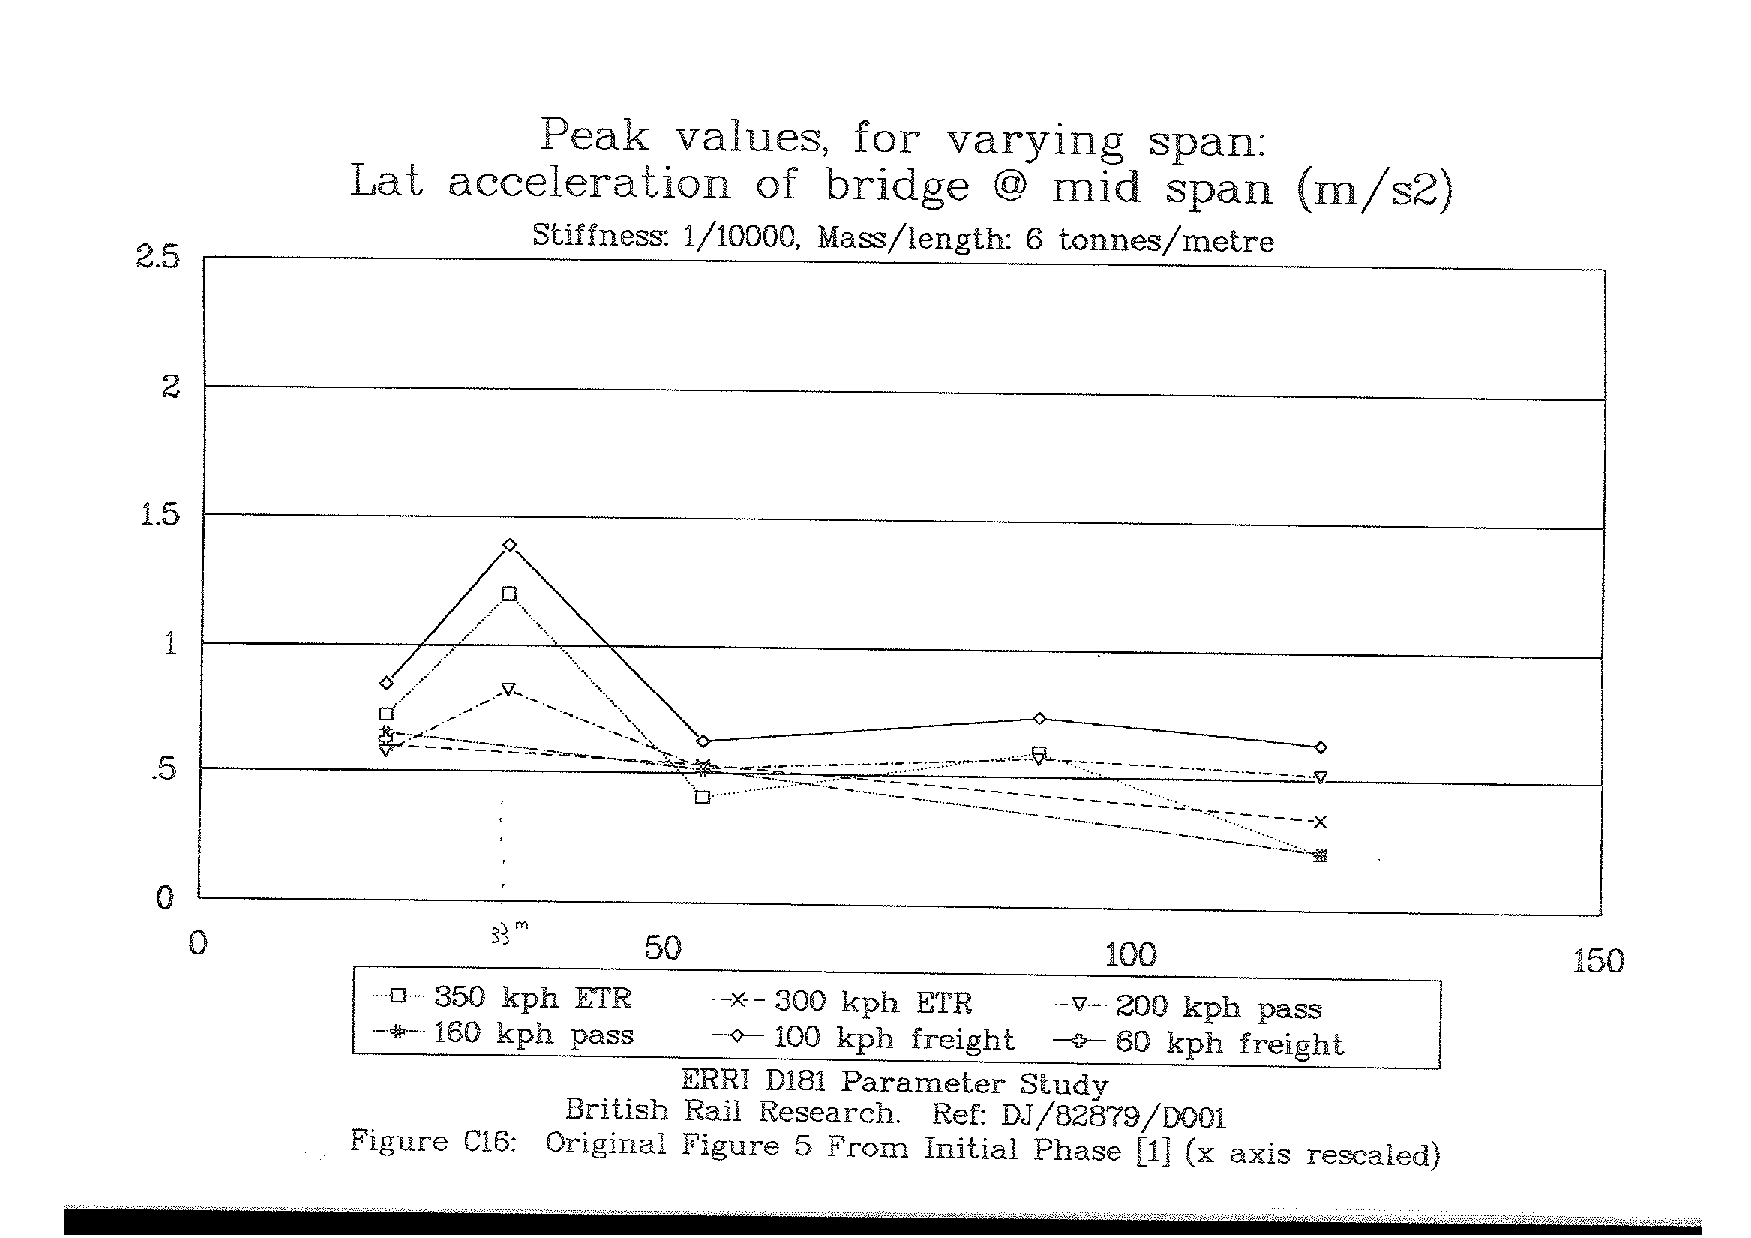
\includegraphics[width=0.8\textwidth]{c16.pdf}
%     \caption{Evidence of resonance caused by kinematic wavelength with span. Extract from \cite[C16]{d181dt329} }
%     \label{fig:c16}
% \end{figure}

% Although wavelength coincidence with span resonance is possible, for longer span bridges (span larger than 50m) it's hardly possible for this type of resonance to build up because the span of the bridge is greater than the wavelength of the train. However, resonance caused by kinematic frequency coincidence with first bending mode is possible even if wavelength and span doesn't match.

% In this report, emphasis is placed on long span bridges, thus resonance cause by kinematic wavelength with span is not investigated due to above reasons. On the other hand, frequencies of kinematic movements of trains will be studied. 

% \section{Conclusion}
% As discussed in Section.\ref{sec:1.2hz} that the origin of natural frequency remains unknown, it is highly doubted that it's actually the frequency range of vehicle suspension system. Rough calculations have been done to study the natural frequencies of the suspension systems of train examples provided in DT 329, proofing all of the frequencies calculated are within a range of 0.3Hz to 1.0Hz. This result mostly overlaps with the frequency range provided by 1.2Hz criterion proposal. 

% If this hypothesis is true, it can also be concluded that D181 committee made a serious mistake in their criterion proposing. Dynamics of the suspension system is only a factor that influence the global dynamic behaviour of a running train, so as track irregularities, train speeds, train layouts, etc. Proposing a criterion based only on natural frequencies of the suspension system is unacceptable. What's more, CEN committee using this proposed criterion in Eurocode 1991-2 was another unconscious mistake.


\chapter{Train vehicles layouts and geometry}



\section{Locomotives}
\subsection{4-axle locomotives}
Generally, the relevant parameters for categorisation of 4-axle locomotives are axle load P (18 t to 22,5 t) and the bogie axle spacing (2,2 m to 3,4 m).

Typically the mass per unit length is less than 6,4 t/m and the distance from the end axle to the end of the nearest coupling plane is greater than 1,9 m

\subsection{6-axle locomotives}

Generally, the relevant parameters for categorisation of 6-axle locomotives are:

\begin{enumerate}[-]
\item the maximum axle load P (18 t to 22 t) in combination with;
\item the distance between axles within a bogie (1,80 m to 2,25 m).
\end{enumerate}

Typically, the mass per unit length (p) is less than 6,4 t/m and the distance from end axle to the end of the nearest coupling plane (a) is greater than 2,1 m.

\section{Passenger carriages}
 
\section{Wheelset and track dimensions}

Generally the track guage is used as a distance measured between the two rails, more specifically the distance between the inside of the railheads measured 14mm below the surface of the rail. By choosing 14 mm the measurement is less influenced by lipping or lateral wear on the rail head and by the radius r = 13 mm of the rail head face. On normal track the gauge is $1435^{+10}_{-3}$ mm with with a maximum gradient of 1:3000. For new track, however, NS apply the following standards:

\begin{enumerate}
\item Mean gauge per 200 m: $1435^{+10}_{-1}$ mm
\item Standard deviation within a 200 m section less than 1 mm
\end{enumerate}

\begin{figure}[h]
\centering
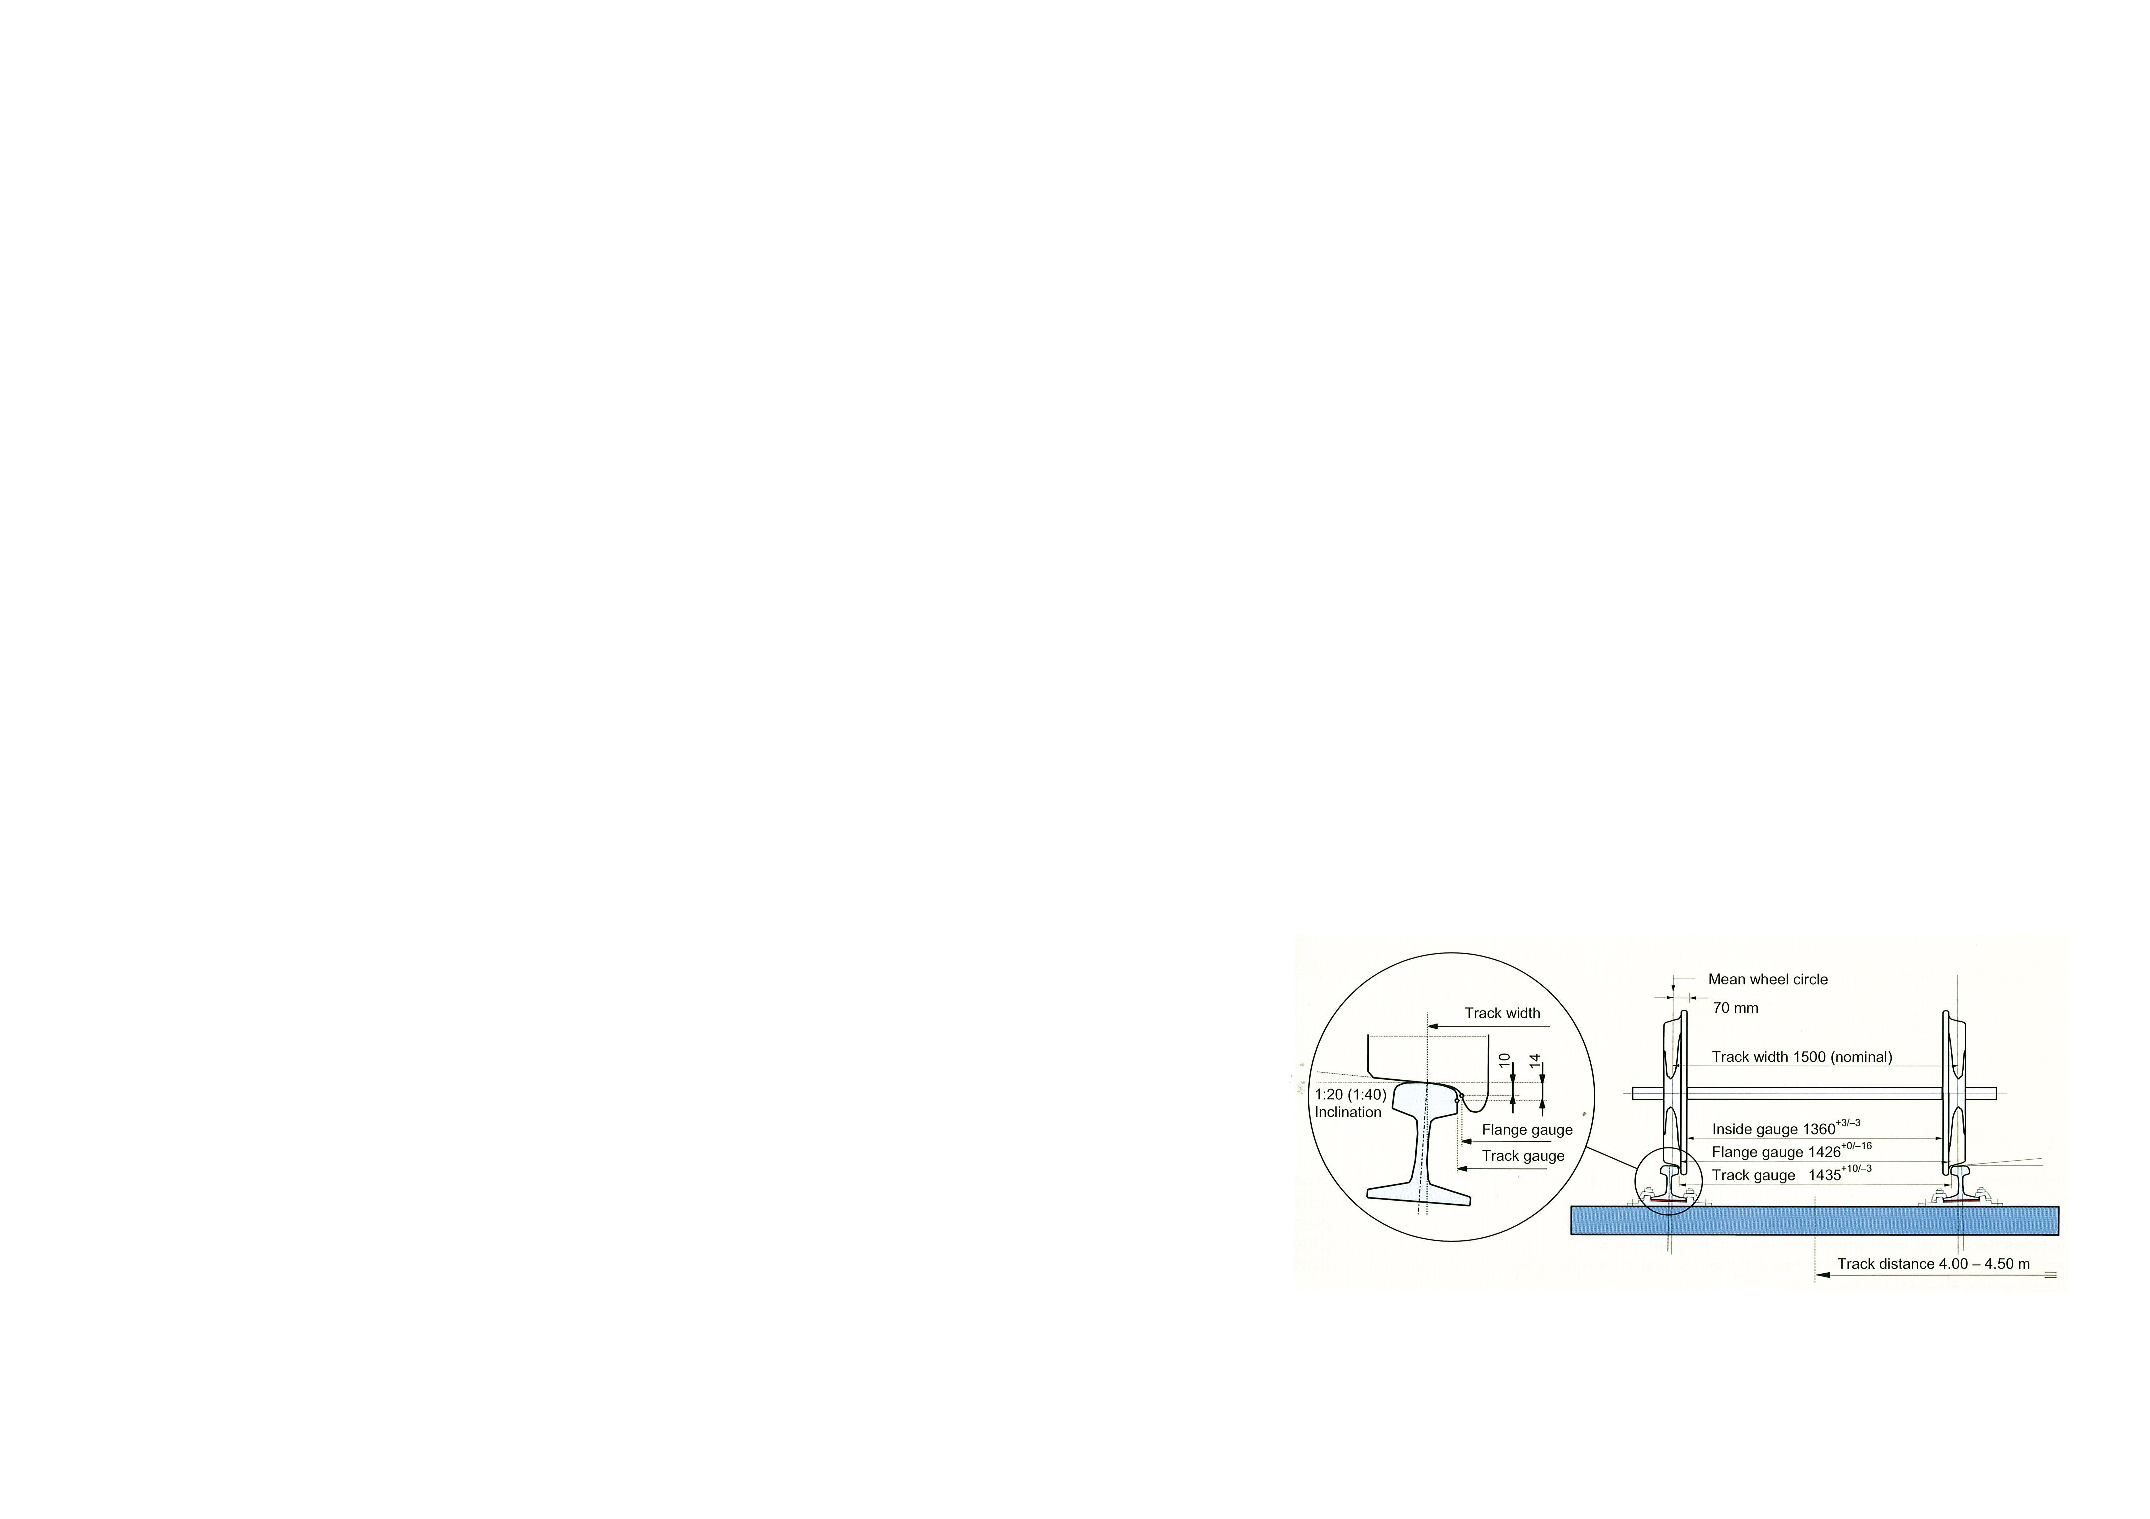
\includegraphics[width=0.8\textwidth]{wheelsettrackdimension.pdf}
\caption{Wheelset and track dimensions for straight normal gauge track. Extracted from \cite[p.17]{esveld2001modern}}
\label{fig:wheelset and track dimensions}
\end{figure}


\section{Conicity and Equivalent Conicity of Wheels}

Originally conical tire profiles with an inclination of 1:20 were used. Since a centrally applied load on the railhead is desired, a rail inclination of 1:20, as shown in Figure 2.1, was also selected; this for instance still applies to NS profile NP 46. UIC 54 rail usually has an inclination of 1:40. This inclination matches the S 1002 worn wheel profile which is in general use in Europe. During manufacturing the tires are given a profile which matches the average shape cause by wear. In contrast to the straight conical profile this has a hollow form.

It is clear that regarding a worn profile the conicity depends on the actual shape of the rail head and tire, including any wear, track gauge, and rail inclination. Likewise, elastic deformation of the wheelset and rail fastenings plays a role.

Generally, the effective or equivalent conicity is defined as:

$$ \gamma_e = \frac{\Delta r}{2y} = \frac{r_1 - r_2}{2y}  $$

Here $r_1 - r_2$ is the instantaneous difference in rolling radius of the wheel treads; generally speaking this is a non-linear function of the lateral displacement y of the wheelset with respect to the central position. The difference between conical and worn profiles is given in Figure.\ref{fig:conicalwornprofiles}. To enable numerical comparisons $\gamma_e$ is determined at a certain lateral displacement $y=\bar{y}$.


\begin{figure}[h]
    \centering
    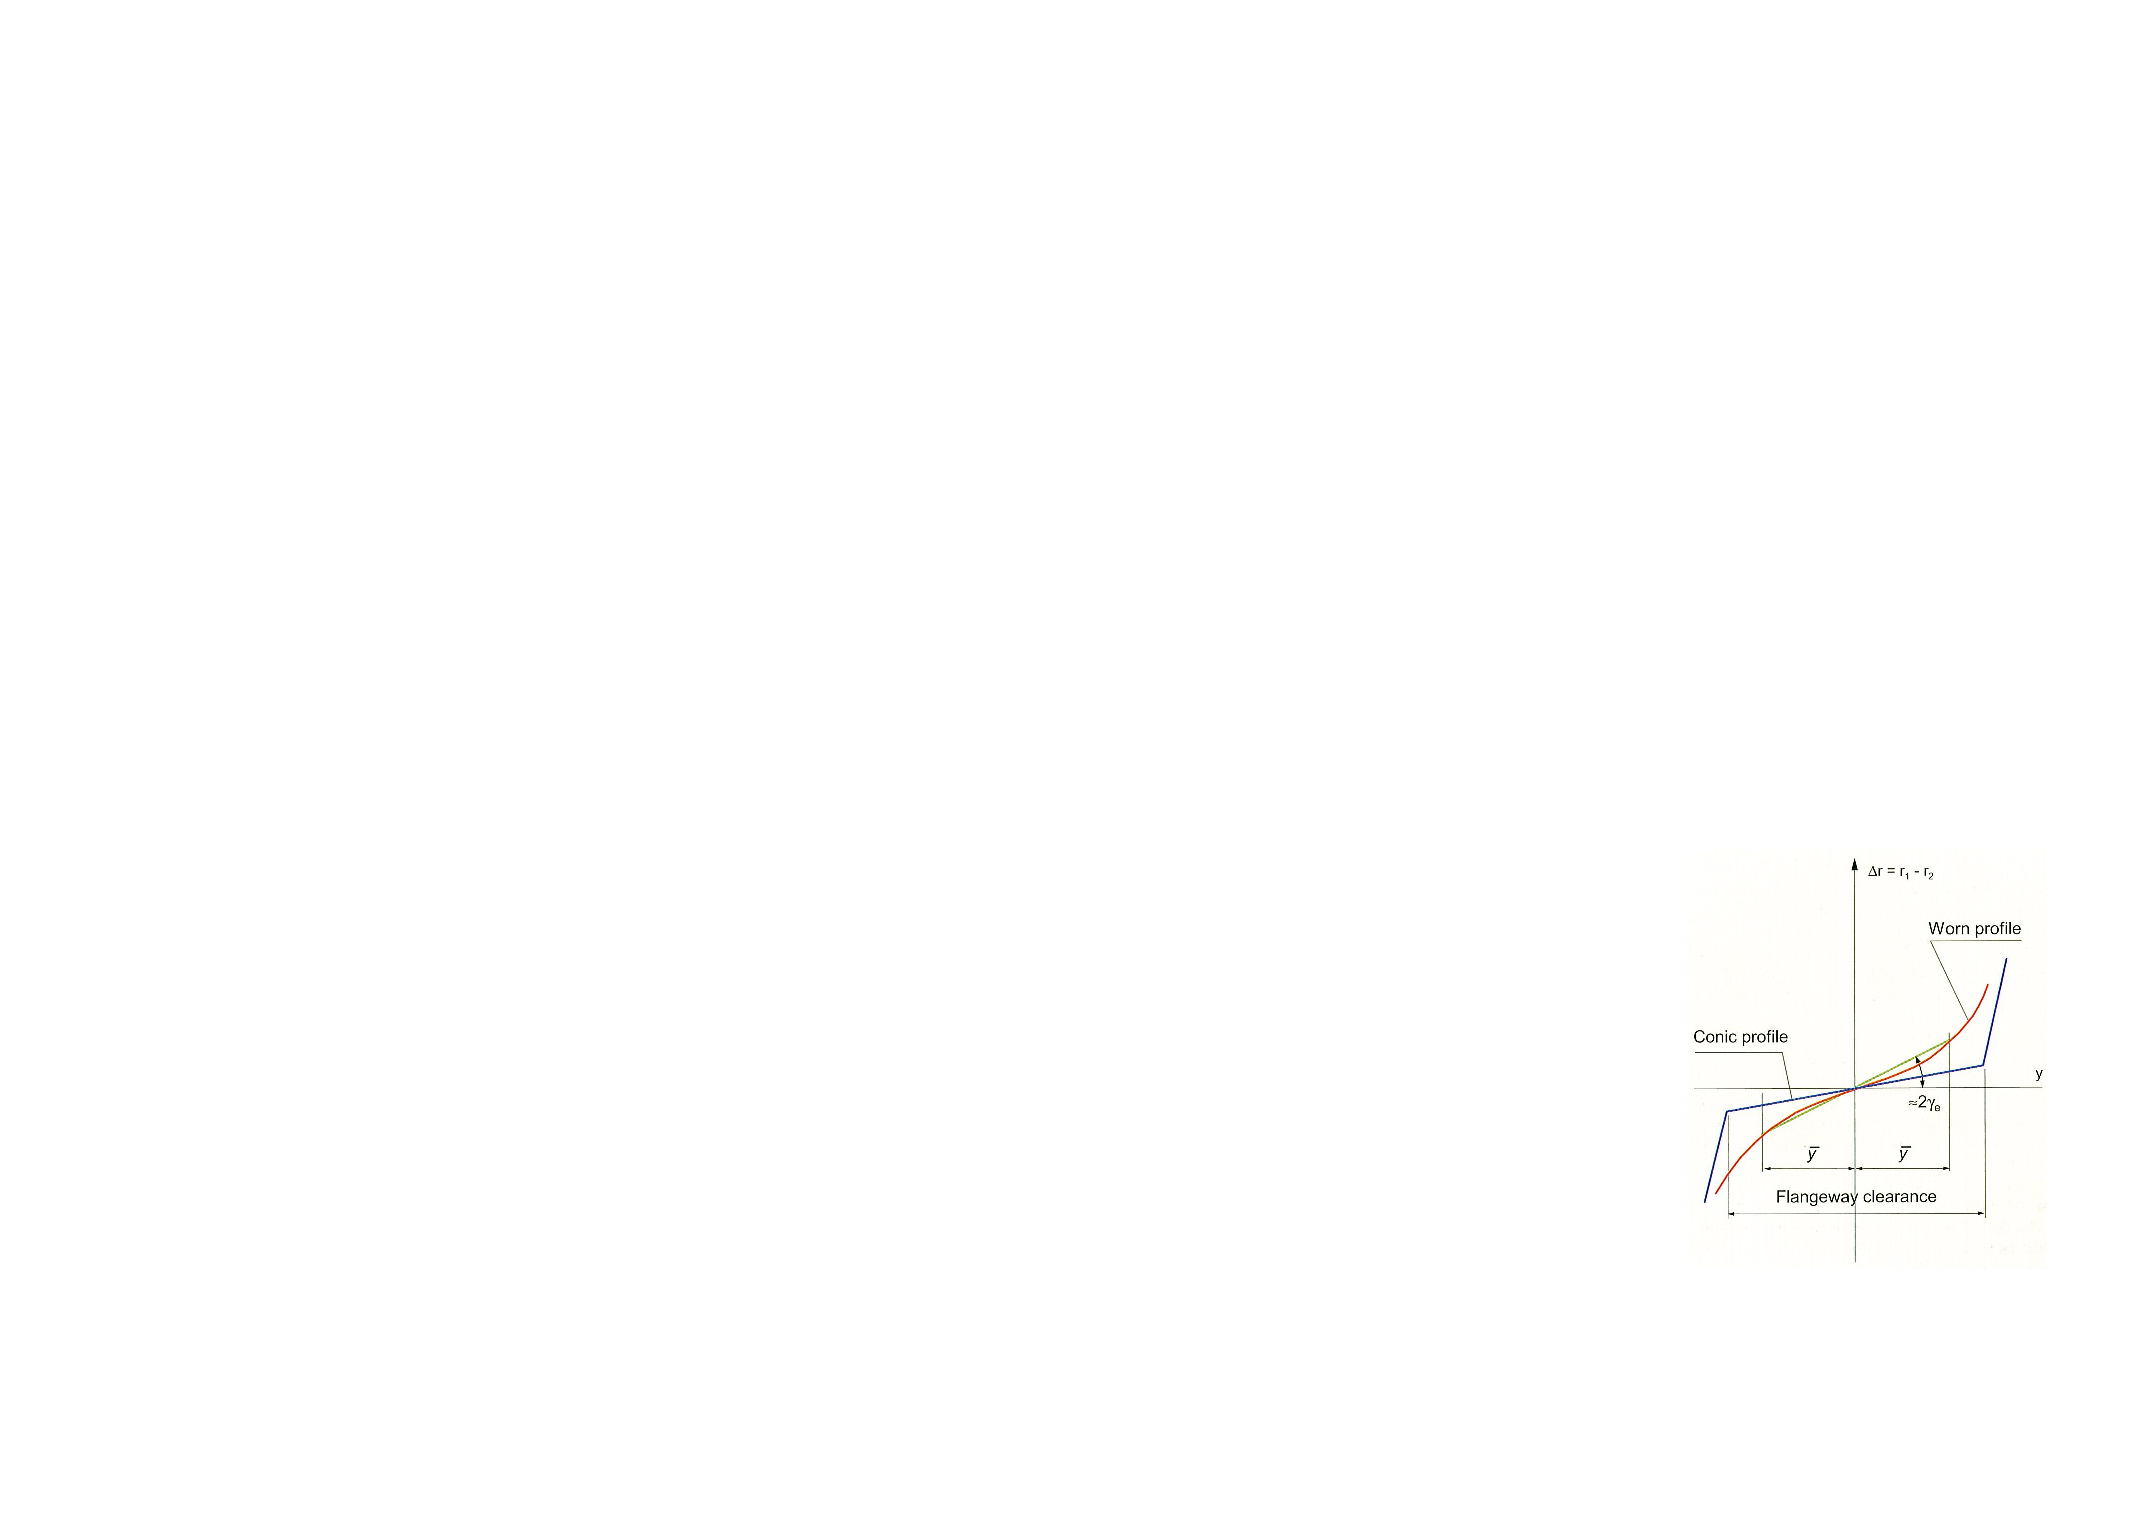
\includegraphics[width=0.6\textwidth]{conicalwornprofiles.pdf}
    \caption{$y-\Delta r$ curves. Difference between conical and worn wheel profiles. Extracted from \cite[2.4]{esveld2001modern}}
    \label{fig:conicalwornprofiles}
\end{figure}

With a conical profile the conicity is constant and above equation becomes:

$$ \gamma_e = \frac{\Delta r}{2y} =\frac{(r+\gamma y)-(r-\gamma y)}{2y} = \gamma $$


\section{Worn wheel profiles}

A perfectly conical wheel profile is unstable as far as its shape is concerned, but will take on a shape that is stable as the effect of wear.

Practical research has shown that over a period of time wheel profiles stabilise with wear at an equivalent conicity of 0.2 to 0.3. With regards to running stability, the equivalent conicity must remain below 0.4 and to ensure the centering effect it must be greater than 0.1.

\section{Trains in Netherlands}

Passenger trains now in service include following models:

\begin{enumerate}
    \item The DD-AR (Dubbeldeksaggloregiomaterieel) \\  EMUs were delivered as DDM-2/3 resembling the bilevel rail cars series DDM-1 from 1985 and operates in fixed formations of 3 or 4 coaches. 4 car trains use a class 1700 locomotive for traction, 3 car trains use an mDDM motorcar, which resembles a DD-AR driving trailer but has electric motors and a single passenger deck on top; the level of this deck is higher than that of a regular single deck rail car, but lower than the upper deck of the other coaches. Three types of coaches are available: Bv (second class), ABv (first and second class) and Bvk (second class driving trailer). The DDM-2/3 series are being modernised from 2010–2013 and after modernisation the series was renamed as NID (Nieuwe Intercity Dubbeldekker).
    \item The VIRM (Verlengd Interregiomaterieel) \\ also called Regiorunner was partially rebuilt from trainsets DD-IRM (Dubbeldeks Interregiomaterieel). DD-IRM was delivered in 3- and 4-car trainsets. 3-car trainsets got one extra coach, 4-car trainsets got two extra coaches. Also, new 4- and 6-car trainsets were built. Thus, a train consists of one or more combinations of 4 or 6 double deck coaches; each combination (multiple unit) has electric motors. More than three hundred coaches are currently operative in the Netherlands.
    \item The Koploper (ICM) (Intercitymaterieel) \\ is a 3- or 4-car multiple unit that when coupled with another one, allows passengers to walk through (the name Koploper being a play on words – literally "head walker", but in actual use meaning "front runner"). The Dutch Railway Company decided to close the heads permanently on 31 October 2005 because the mechanism broke down too often. A scheduled modernisation of around 7 million euro will see the ICM fleet updated. The renovated ICM trains provide 13\% more seats (reducing the leg room to uncomfortable small for the long haul journeys they serve in 2nd class, which is further aggravated by a waste bin that is placed on the backsides of the seats in front), have a new interior, a bathroom accessible by wheelchairs, airconditioning as well as upgrades to the engine and connection systems. The head doors are removed. Also, these (renovated) trains are the first trains in the NS fleet equipped with OBIS. OBIS provides a (free) WiFi-connection on board, along with in-train journey information provided through screens and (automated) vocal announcements through the trains speakers. This journey information provides the actual status, and thus is always up-to-date to the actual situation this trip, and the stations is passes.
    \item The Sprinter (SGM, Stads Gewestelijk Materieel) \\ is a two or three car electric, used on small distances. They are named Sprinter because they're able to accelerate and brake quite fast, making them very suitable for 'stoptrein' services. They were also specifically designed for urban environments where they run commuter services. As a result, they are most commonly found in the Randstad area. The initial idea was that the Sprinter would provide somewhat of a subway/metro service but this plan failed as the cities of Amsterdam and Rotterdam continued to construct their own rapid transit systems. Nevertheless, in the densely populated Randstad, the Sprinters remain popular. Two car versions were revised and renamed to Citypendel. All Sprinters are now refurbished into the new white/yellow/dark blue livery.
\end{enumerate}

All of passenger train coaches have a wheel diameter of 920 mm. 

Locomotives of freight trains have wheel diameter of 1000 mm.

\section{Lateral Track Irregularities}
This section describes allowable lateral track irregularities defined in EN13848-5\cite{13848}. 

Lateral alignment irregularities was defined in EN13838-1. It states:"Deviation $y_p$ in y-direction of consecutive positions of point P... on any rail, expressed as an excursion from the mean horizontal position (reference line) covering the wavelength ranges stipulated below and calculated from successive measurements ...". See Figure \ref{fig:lateraldeviationdefine}.

For lateral deviations, the following wavelengths shall be considered: $D1 = 3 -25 m$, $D2 = 25 - 70 m$ and $D3 = 70 - 200 m$. 

\begin{figure}[h]
    \centering
    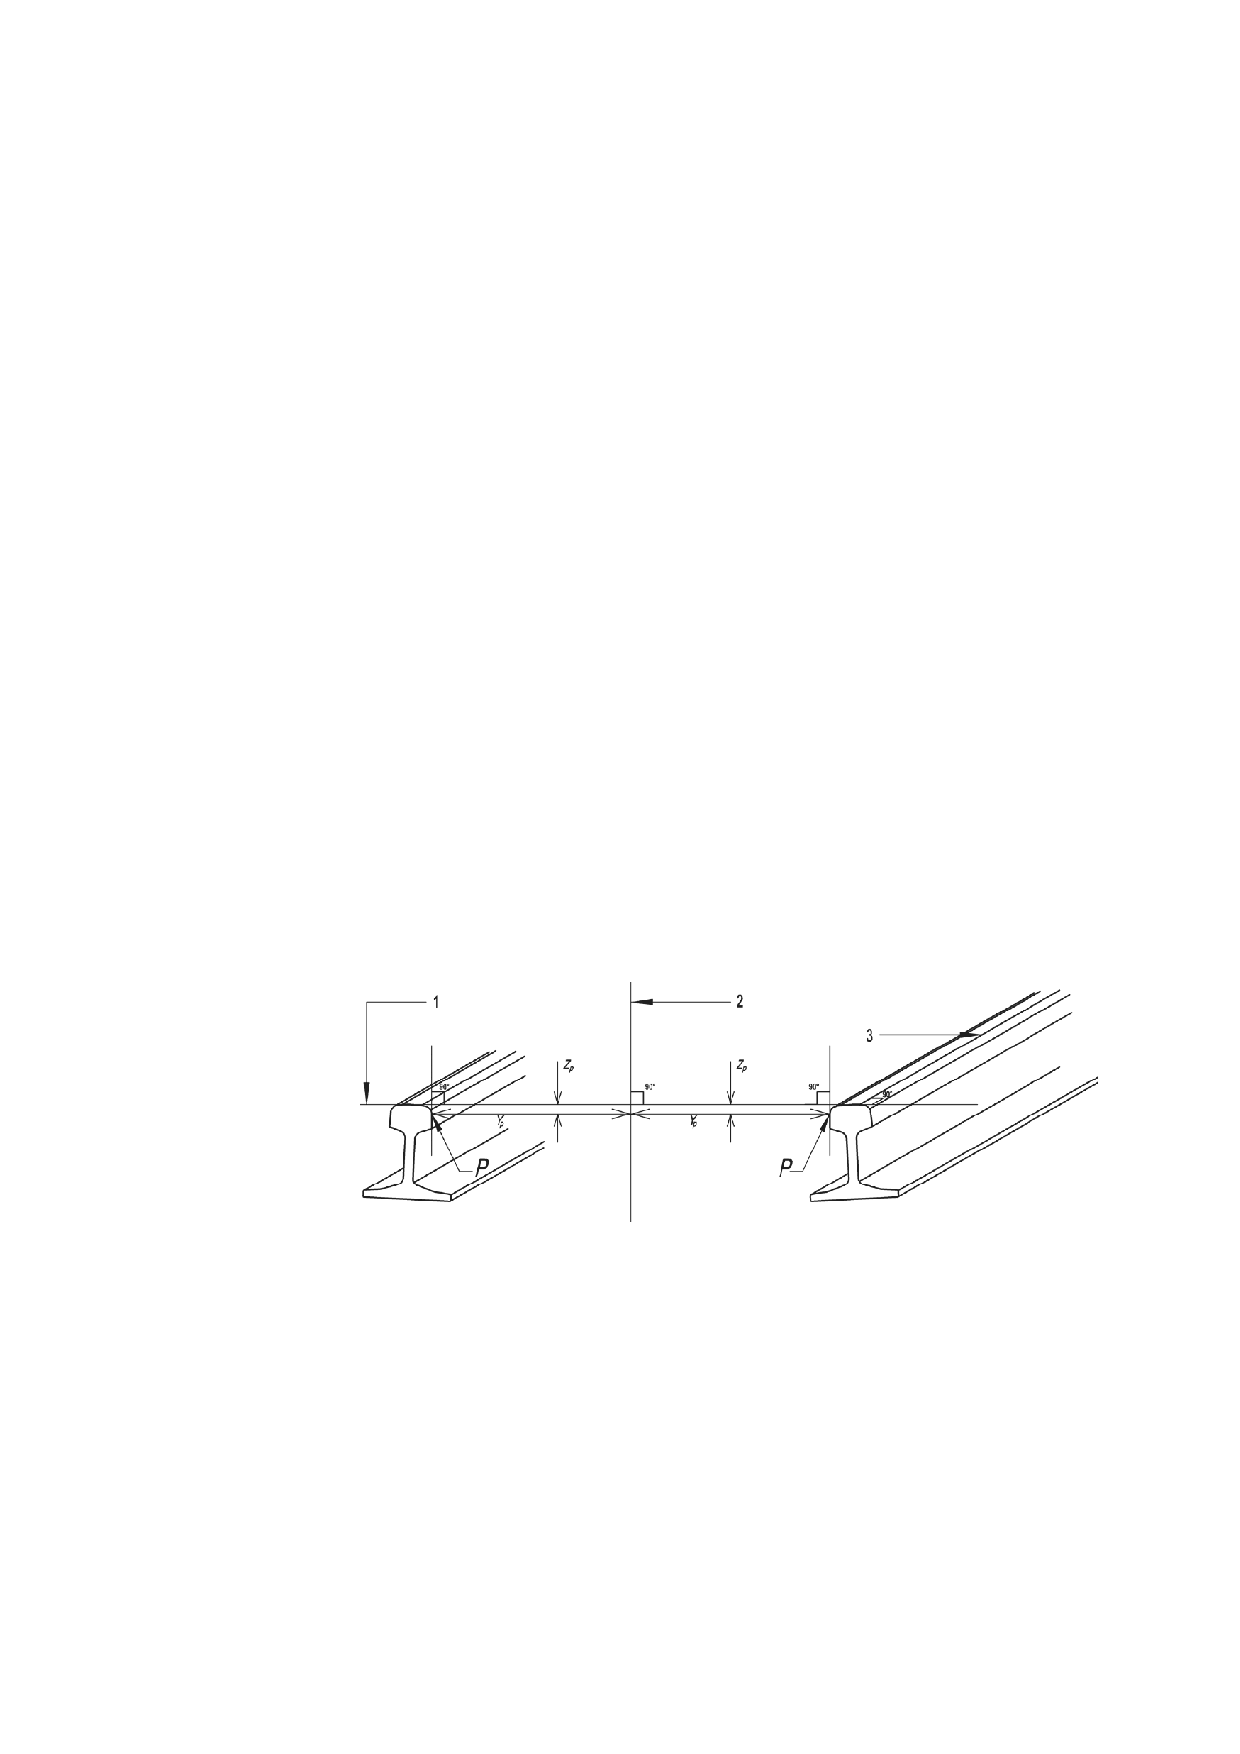
\includegraphics[width=0.8\textwidth]{lateraldeviationdefine}
    \caption{Lateral deviation definition. Lateral deviations $y_p$ for each rail with 1: running surface, 2: reference line and 3: centre line of running table}
    \label{fig:lateraldeviationdefine}
\end{figure}

Table \ref{tab:lateraldeviation} defines the allowable standard deviation for lateral track irregularities.

\begin{table}[h]
    \centering
    \caption{Alignment - AL - Standard deviation. Extracted from \cite[Table B.6]{13848}}
    \begin{tabular}{cc}
        \hline
        Speed(km/h) & Standard deviation(mm) \\
        \hline
        $V\leq 90$ & 1.5 to 1.8 \\
        $80 < V \leq 120$ & 1.2 to 1.5 \\
        $120 < V \leq 160$ & 1.0 to 1.3 \\
        $160 <V \leq 230$ & 0.8 to 1.1 \\
        $230 <V \leq 300$ & 0.7 to 1.0 \\
        \hline
    \end{tabular}
    \label{tab:lateraldeviation}
\end{table}


\chapter{Parametric Study}
% The objective of parametric study is to observe lateral vibration frequency range of different trains types. Due to limited source of reliable vehicle data, train modelled in this study is the same train data used in ERRI Report RP6\cite{d181} where necessary. Considering effects that was assumed to have been taken into account by ERRI in previous chapter, following parameters to be checked are determined. 

% Parameters to be examined:
% \begin{enumerate}
% \item different layouts
% \item suspension system stiffness
% \item mass of the train
% \item track irregularities
% \item bridge span
% \item bridge mass
% \item bridge stiffness
% \end{enumerate}


% To assess the effects of different parameters on train lateral frequency, following parametric study using FEM software are conducted. Please note that by default, the loading of every single axle is 22.5t, according to the maximum allowable axle load defined in \cite{EC15528}

% The process will start from comparably easy models then develop them into more sophisticated ones. With the development of the models, effects will be added into account one by one. Details of modelling will be described in following sections.

% \section{Basic phenomenon modelling}
% Phenomenon to be modelled: kinetic movement. track irregularities impact. 
% The aim of modelling is to reproduce FEM analysis by VAMPIRE software done by ERRI D181 committee in 1996. 

% Complicated simulation of vehicle-structure system is broken done into more basic modules. The order of modelling is shown in Fig.\ref{fig:modellingsequence}. More sophisticated model develops basing on simpler ones to minimize the appearance of errors. 

% \begin{figure}[h]
%     \centering
%     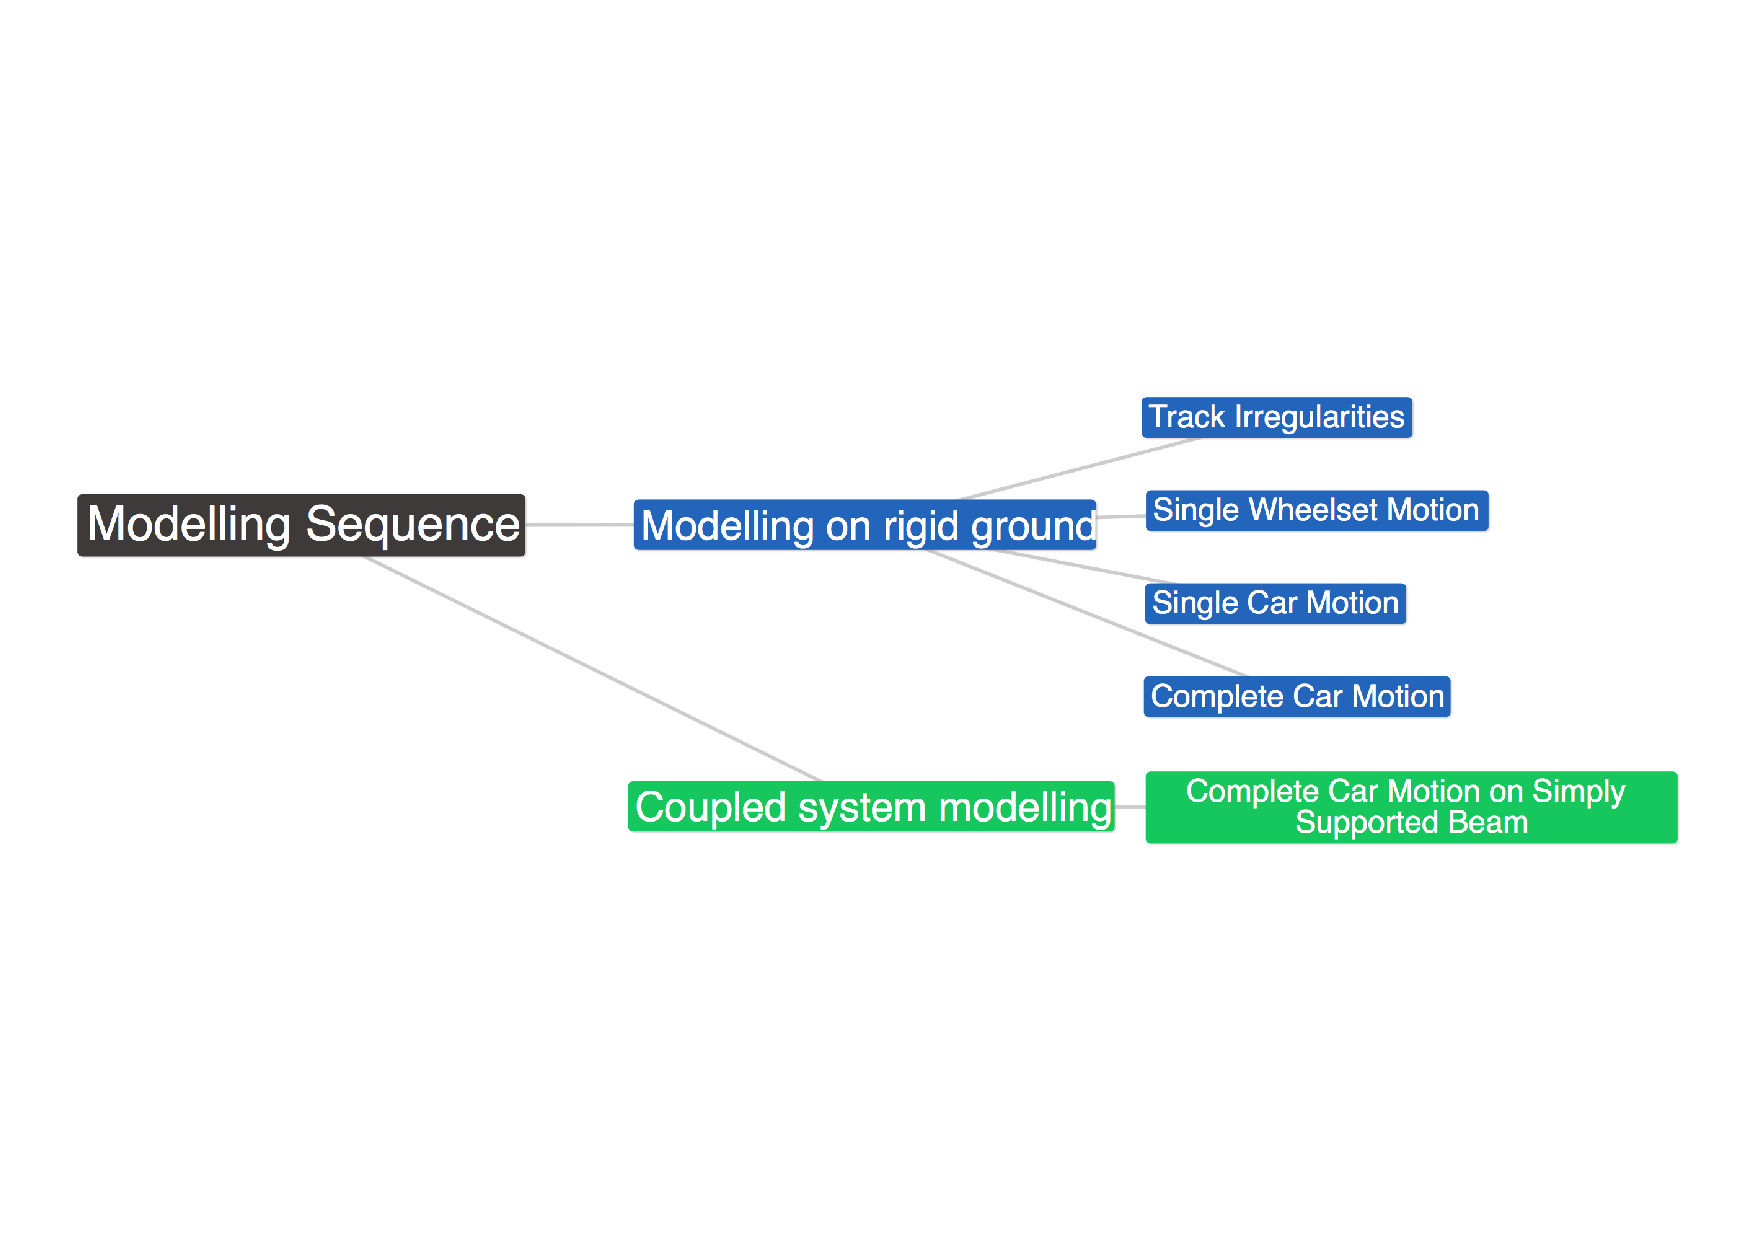
\includegraphics[width=0.8\textwidth]{modellingsequence.pdf}
%     \caption{Modelling sequence}
%     \label{fig:modellingsequence}
% \end{figure}


% \subsection{Track irregularities profile modelling}
% Trying to find a way of introducing track irregularities into the current model
% Track irregularities are small imperfections cause by manufacturing, train running, etc. Sample track irregularities over a certain length of track can be measured, as well as numerical generated. Track irregularities is the first effect to be modelled because it is the exciting source of other train lateral dynamic effects.

% An example of numerically generated track irrgularity profile is illustrated in Fig.\ref{fig:trackirregularities70_120}

% \begin{figure}[h]
%     \centering
%     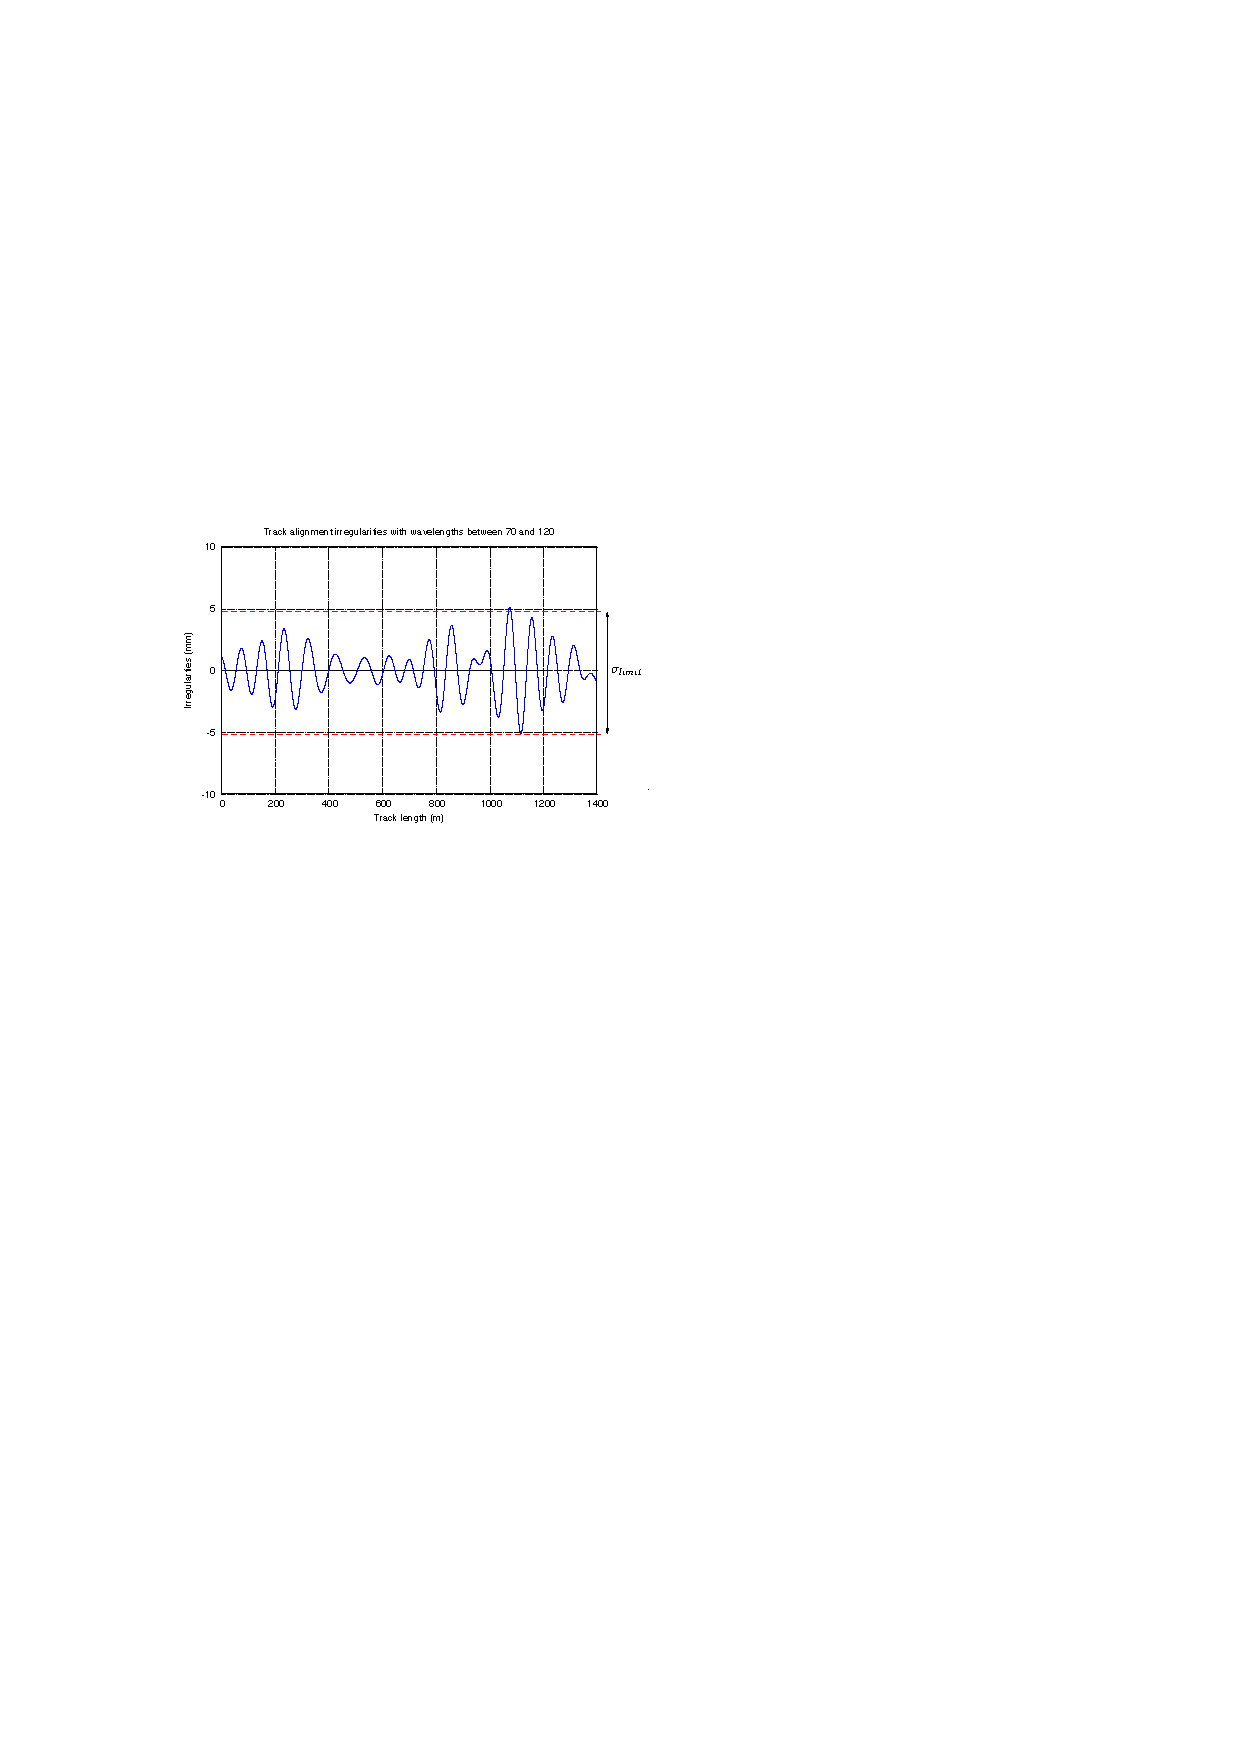
\includegraphics[width=0.8\textwidth]{trackirregularities70_120.pdf}
%     \caption{Track alignment irregularities with wavelengths between 70 and 120. Extracted from \cite{dias2008study}}
%     \label{fig:trackirregularities70_120}
% \end{figure}



% \subsection{Kinetic movement of single wheel-set}
% This step is to reproduce and evaluate the reliability of a basic wheelset-track model. The result of this model will be compared with Klingel formula.

% To be noted: Klignel kinematic movement description makes a number of simplifying assumptions since it neglects forces. For one, it assumes that the rolling resistance is zero. A wheelset (not attached to a train or truck), is given a push forward on a straight and level track. The wheelset starts coasting and never slows down since there are no forces (except downward forces on the wheelset to make it adhere to the track and not slip). But in the FEM model forces will be included to pave the way for following analyses.

% Research showed that Klingel's formula coincides well with measured data from experiments. This proves that if the result of this simulation coincides with what Klingel formula predicted, the model is reliable.

% This wheel-set will move on rigid and fixed tracks.

% Some thoughts:
% I need to model simplified contact stress, but due to unknown friction force, how do I maintain constant speed of train?

% \begin{figure}[h]
%     \centering
%     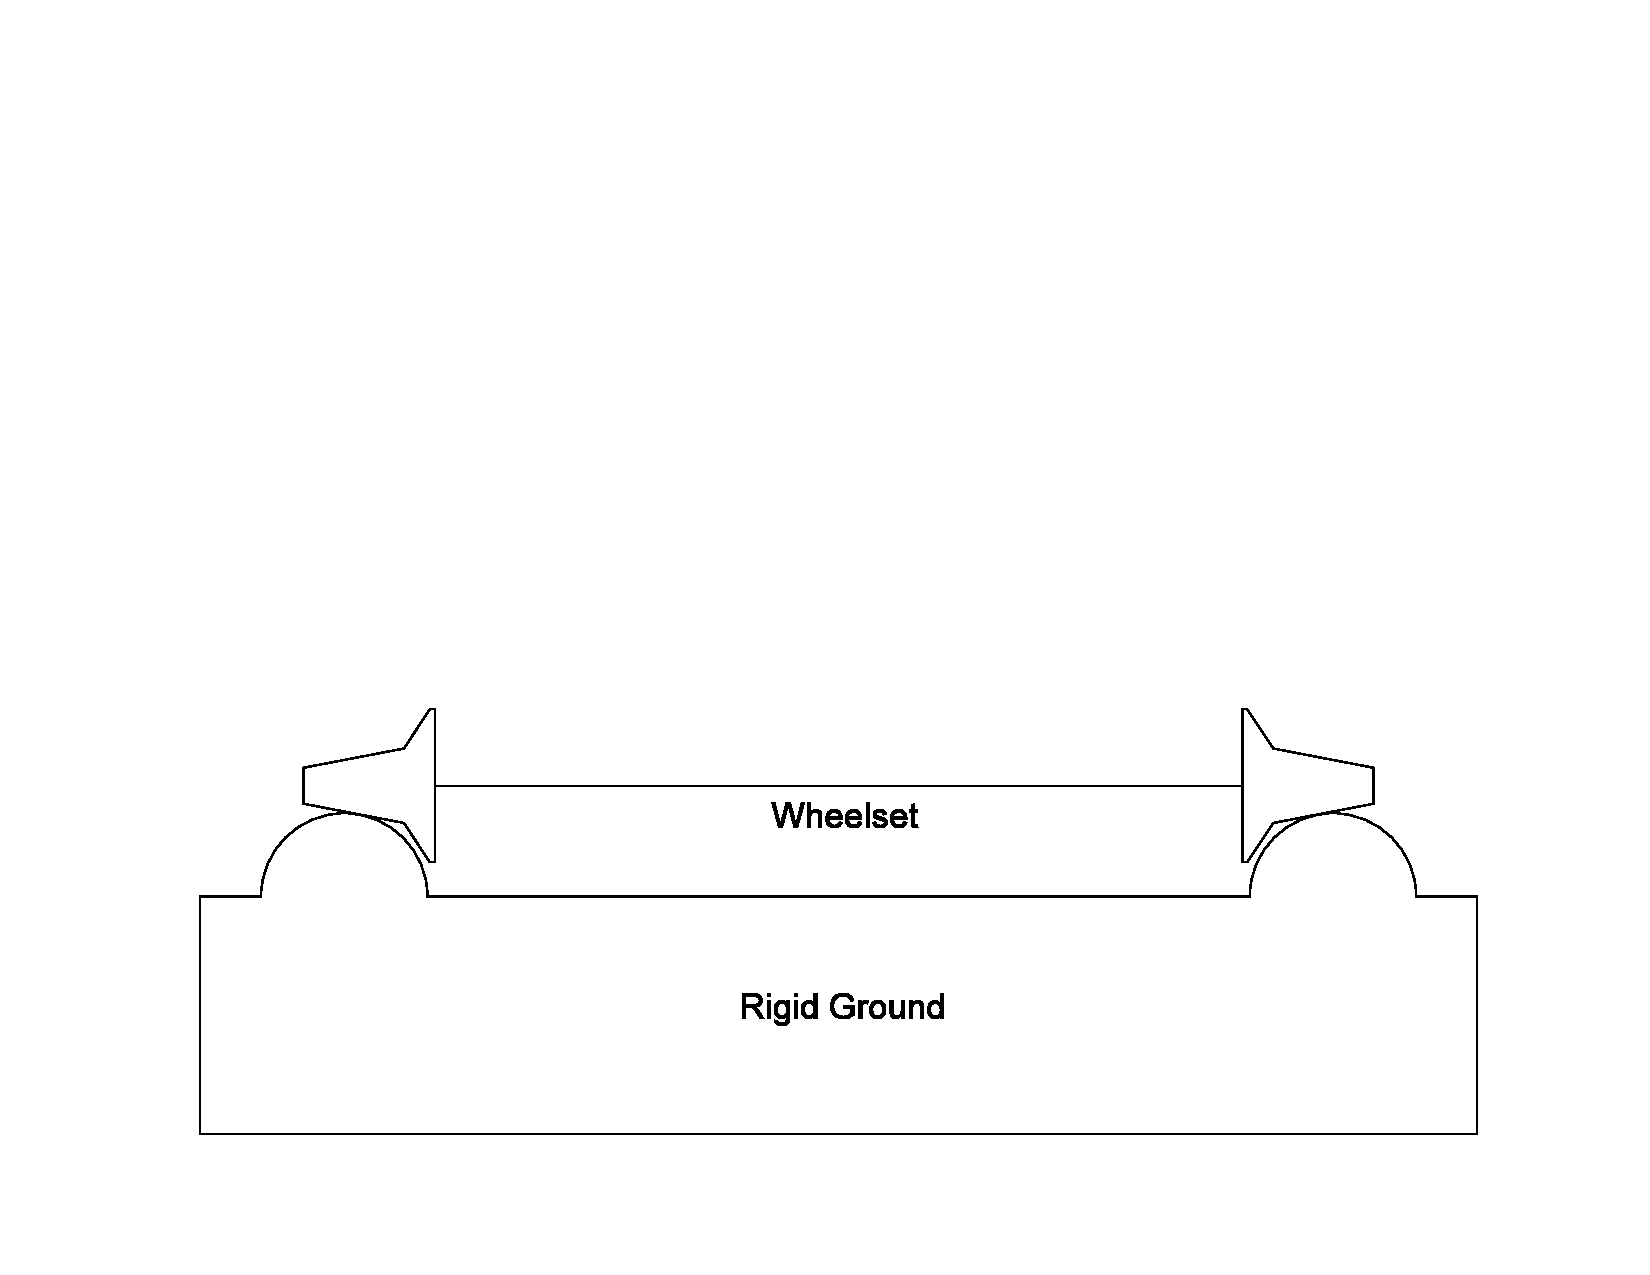
\includegraphics[width=0.5\textwidth]{wheelsetmodel.pdf}
%     \caption{Wheelset movement model}
%     \label{fig:wheelsetmovementmodel}
% \end{figure}

% \begin{figure}[h]
%     \centering
%     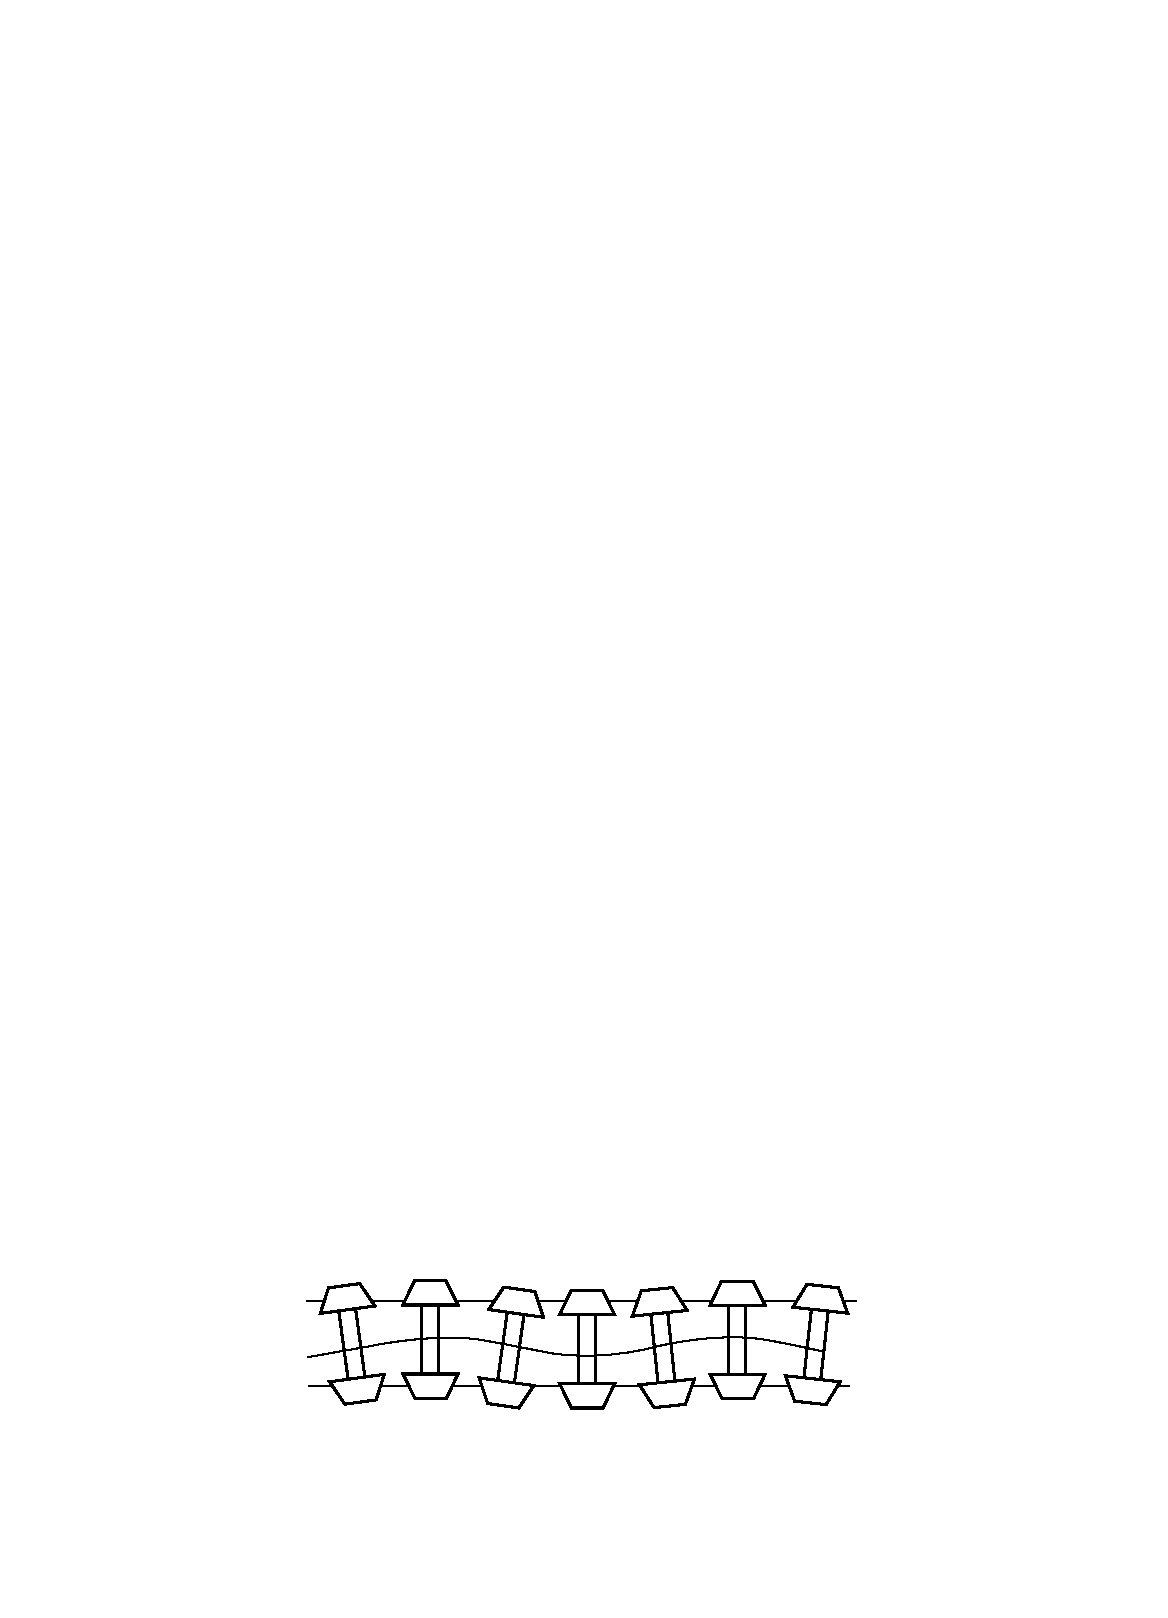
\includegraphics[width=0.8\textwidth]{singlewheelset.pdf}
%     \caption{Single wheel set kinetic oscillation view from top}
%     \label{fig:singlewheelset}
% \end{figure}


% \subsection{Kinetic movement of single car}
% This step is to add more sophisticated mass-spring system attached to the single wheel-set model in previous section. The mass-spring system represents the suspension system of cars in lateral direction. However, since the data to be used is the same data used in 1996, using more up-to-date train data is suggested for future researches.

% Several car types will be input including locomotives, passenger car and freight car.

% The car will move on flexible and fixed tracks. 

% \begin{figure}[h]
%     \centering
%     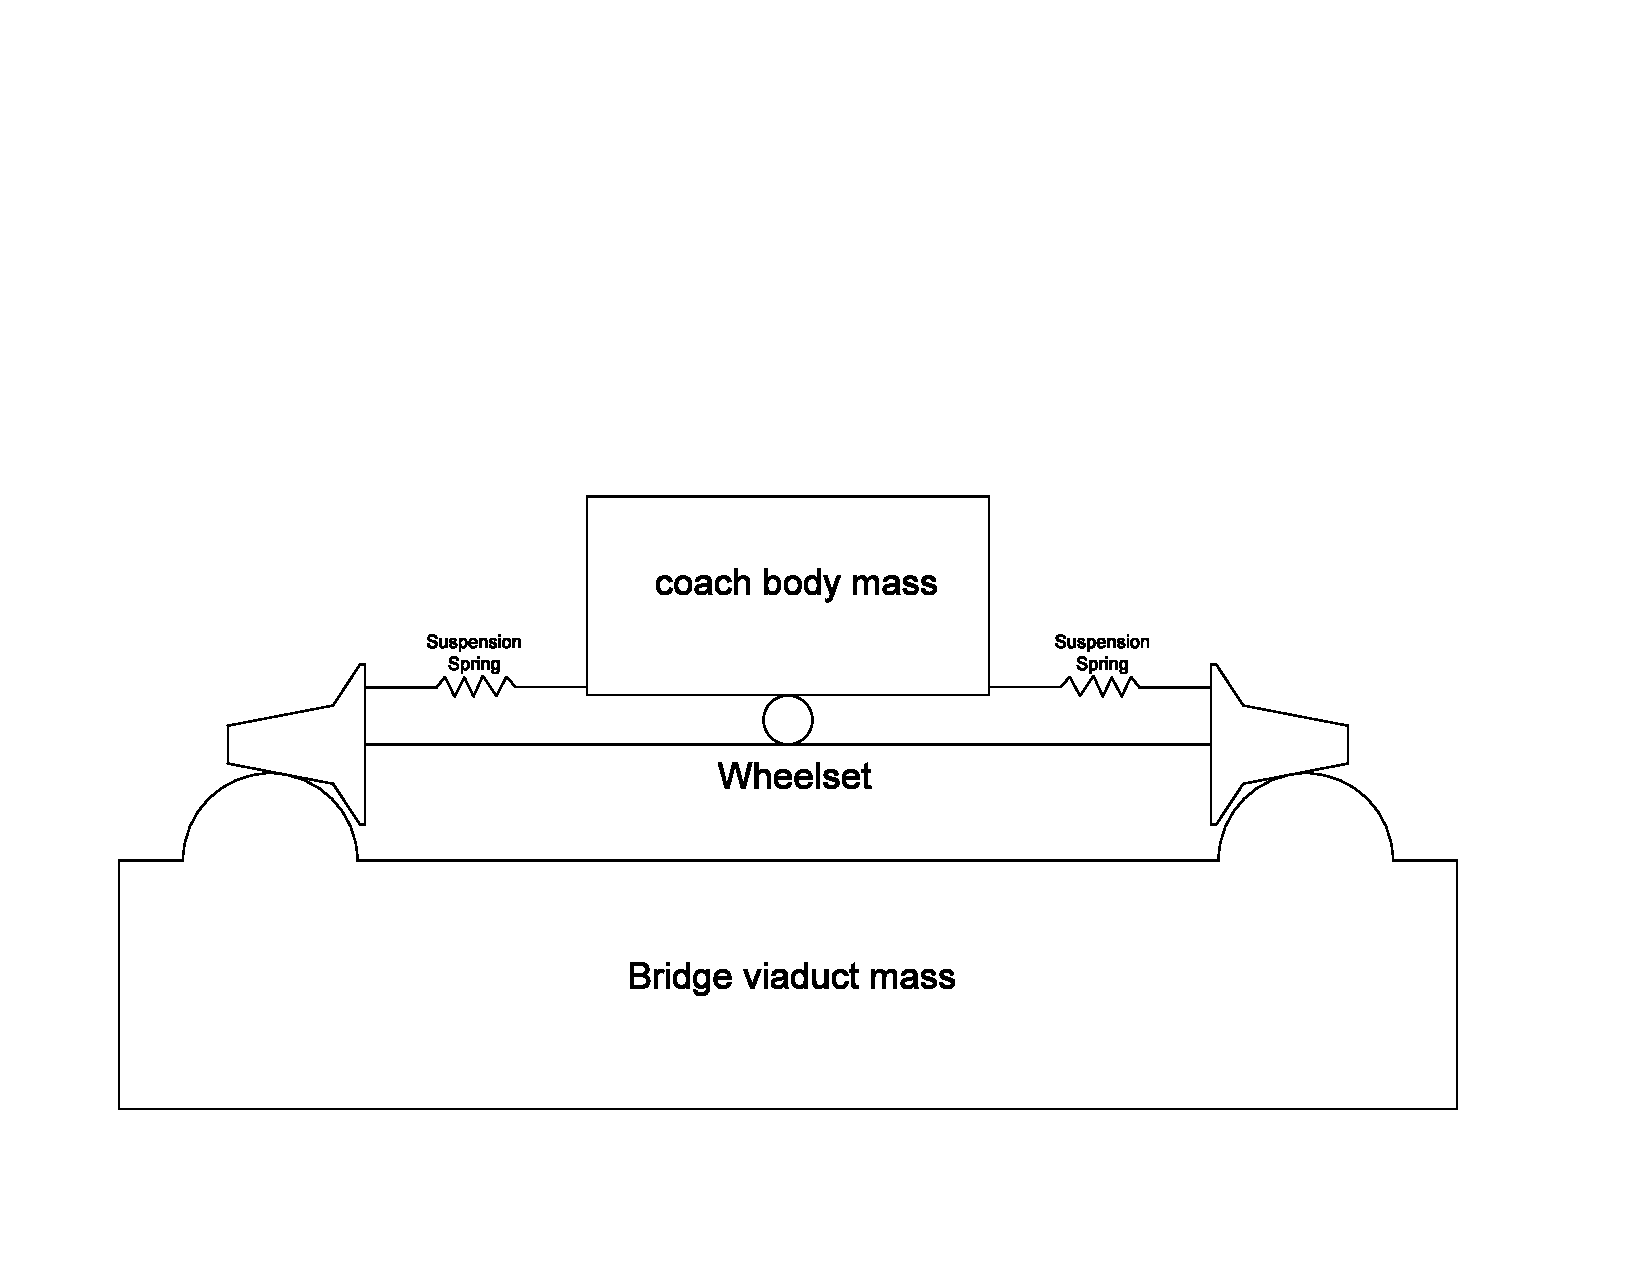
\includegraphics[width=0.5\textwidth]{trainmodellongwheelprofile.pdf}
%     \caption{Sample view of one single car model model used in FEM software from the front}
%     \label{fig:trainmodellong}
% \end{figure}

% \begin{figure}[h]
%     \centering
%     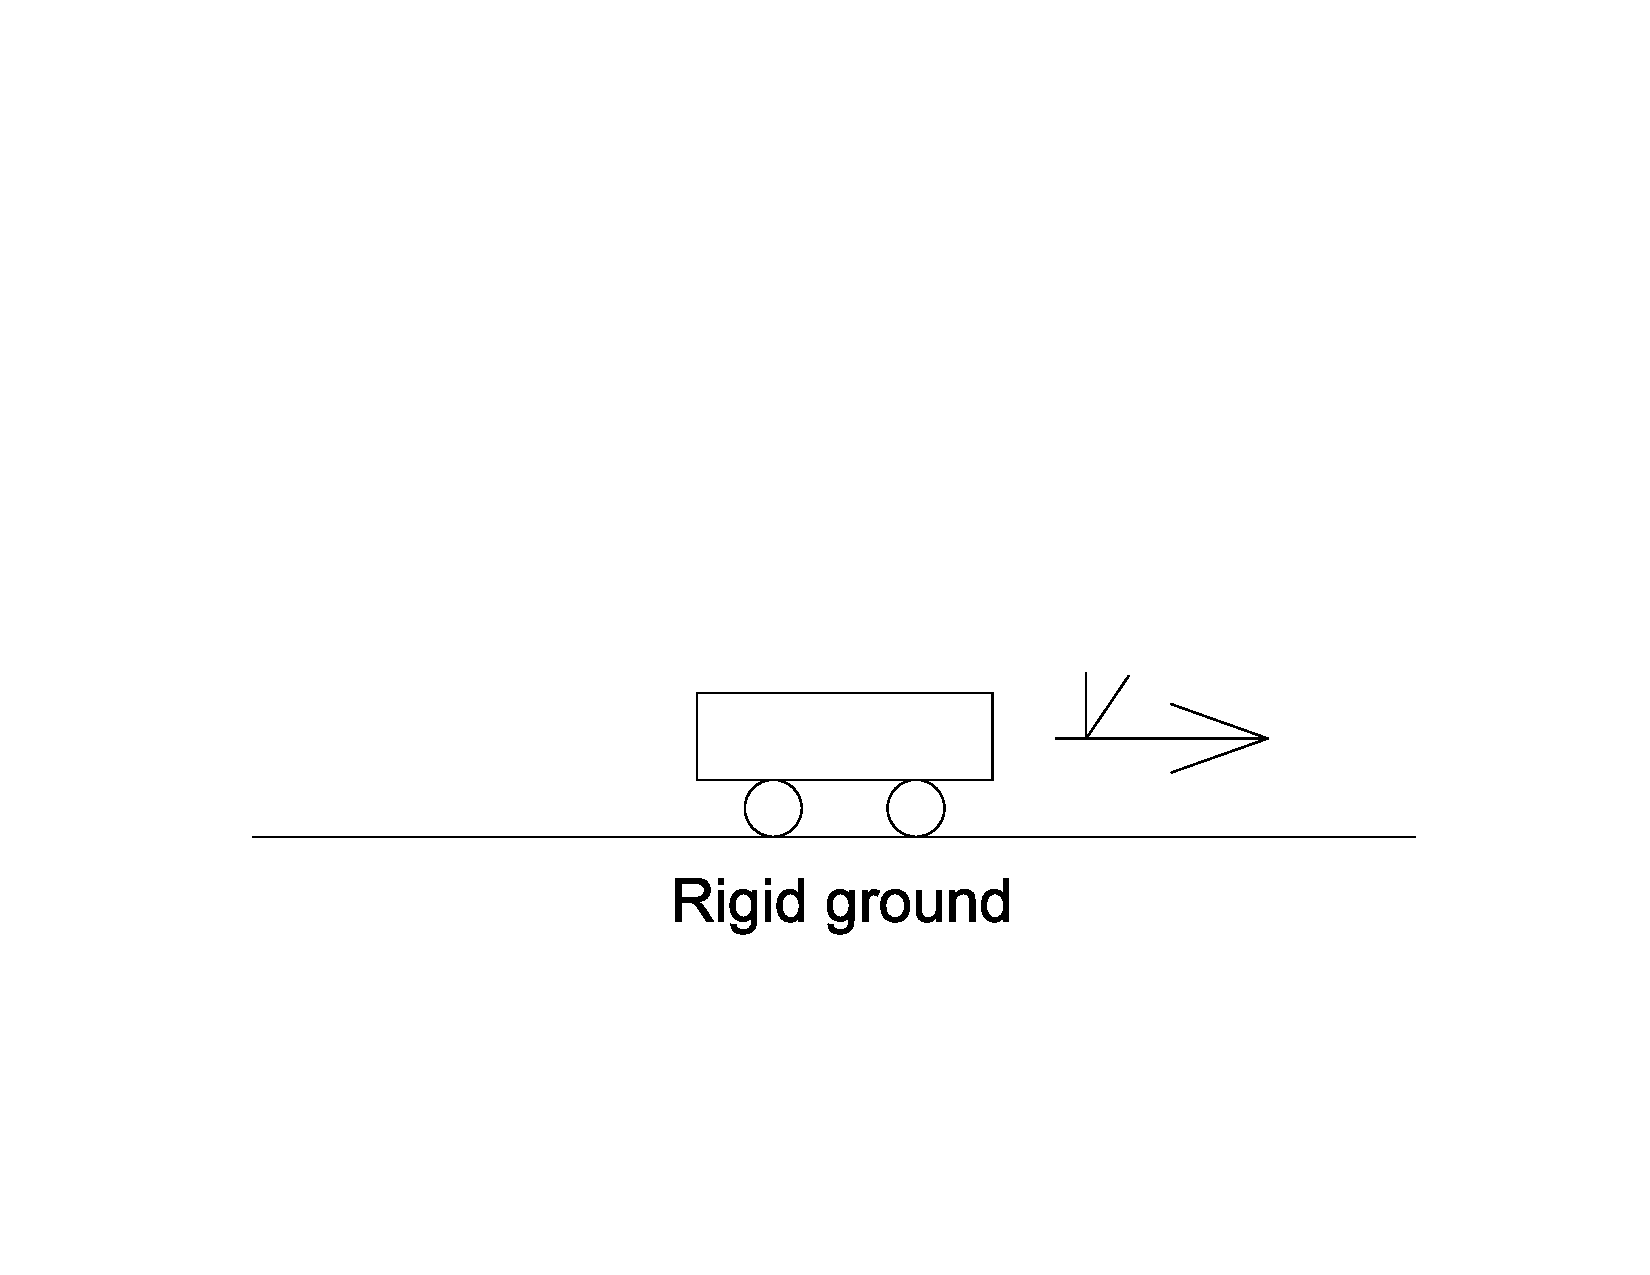
\includegraphics[width=0.8\textwidth]{trainmodellateralsimple.pdf}
%     \caption{Car model on rigid ground}
%     \label{fig:trainmodellateralsimple}
% \end{figure}

% An example of table of suspension parameters is listed in Fig.\ref{fig:suspensiondata}:

% \begin{figure}[h]
%     \centering
%     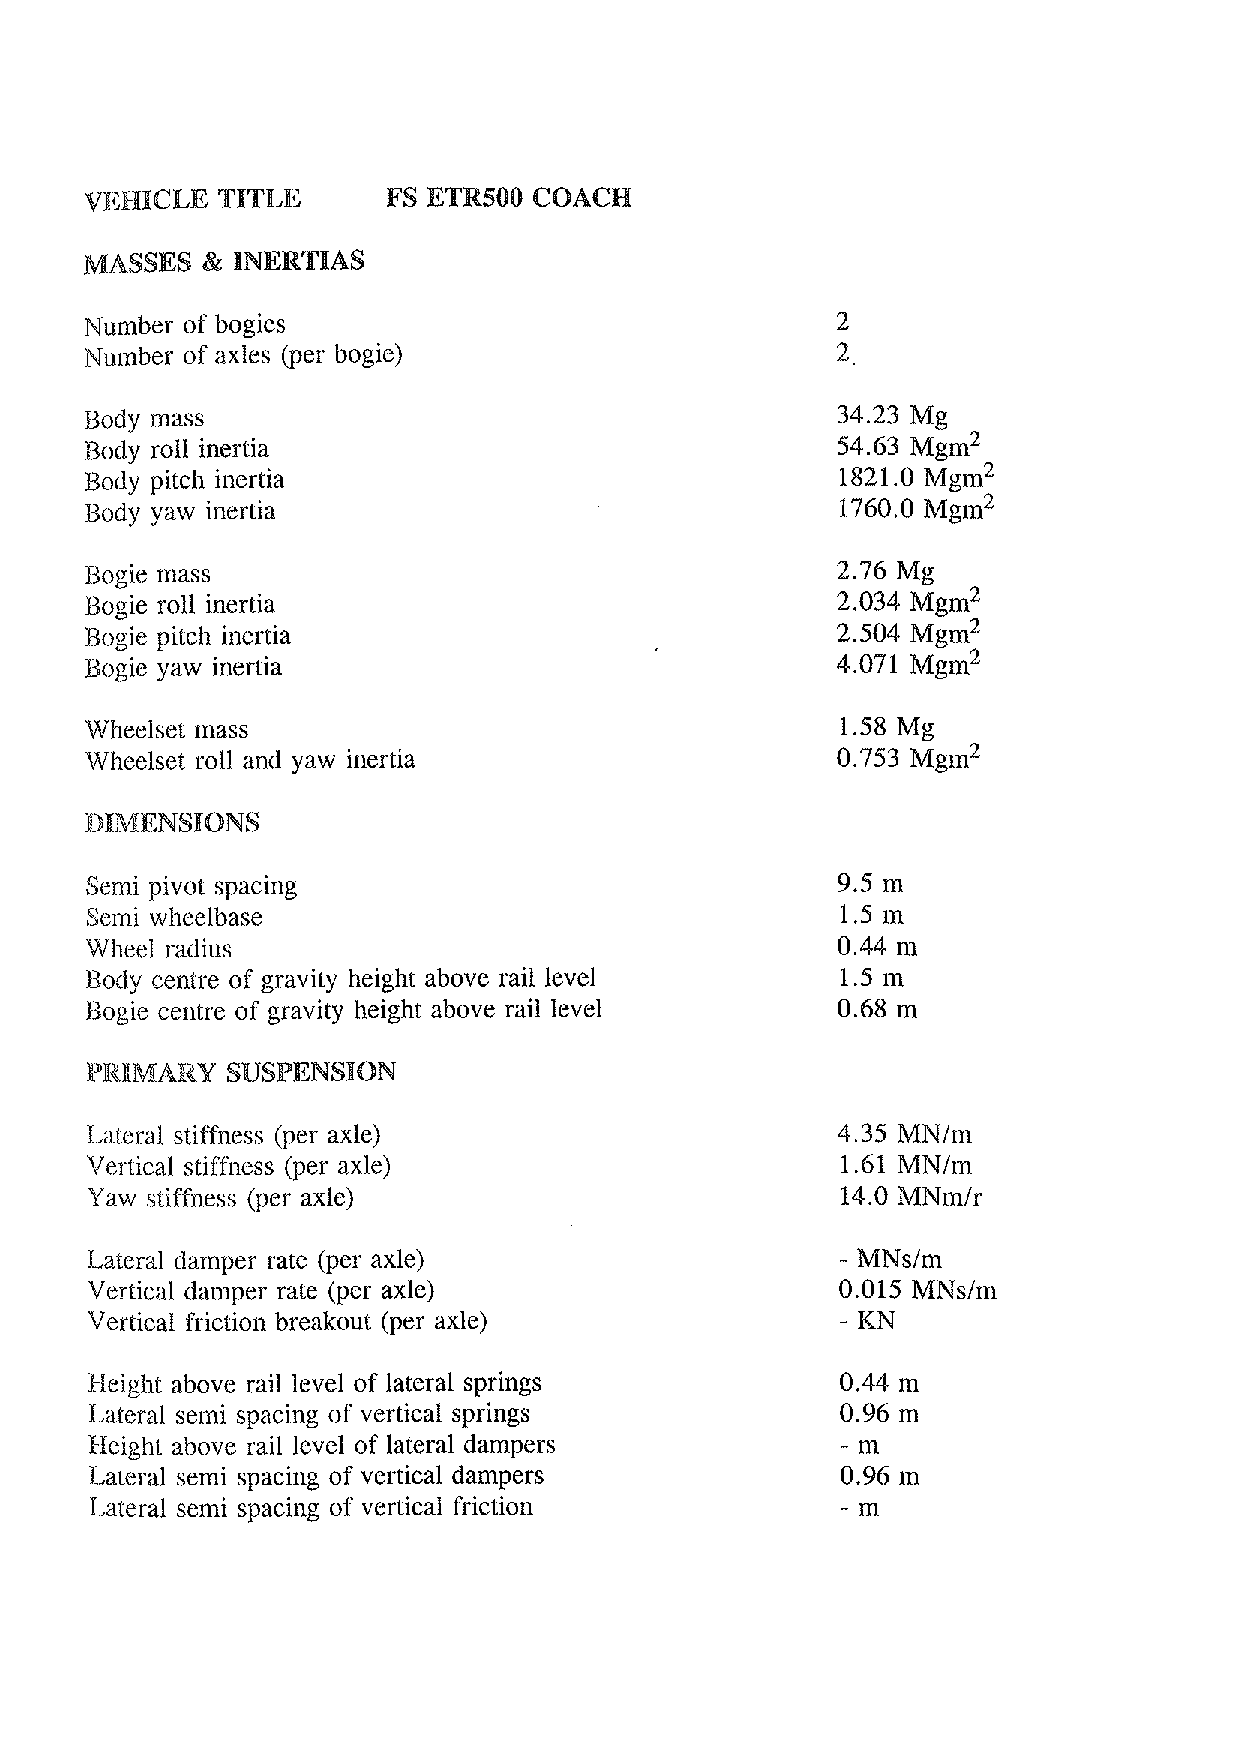
\includegraphics[width=0.8\textwidth]{suspensiondataexample.pdf}
%     \caption{example of table of suspension parameters extract from RP6\cite{d181}}
%     \label{fig:suspensiondata}
% \end{figure}

% Other parameter tables used are included in the appendix.

% \subsection{Kinetic movement of complete train}
% This step is to assemble car models defined in previous steps, trying to find out the influence of axle layouts on lateral frequency of single wheelset. Assemble rules are according to \cite{EC15528}. 

% The connections between cars are hinged. 

% \begin{figure}[h]
%     \centering
%     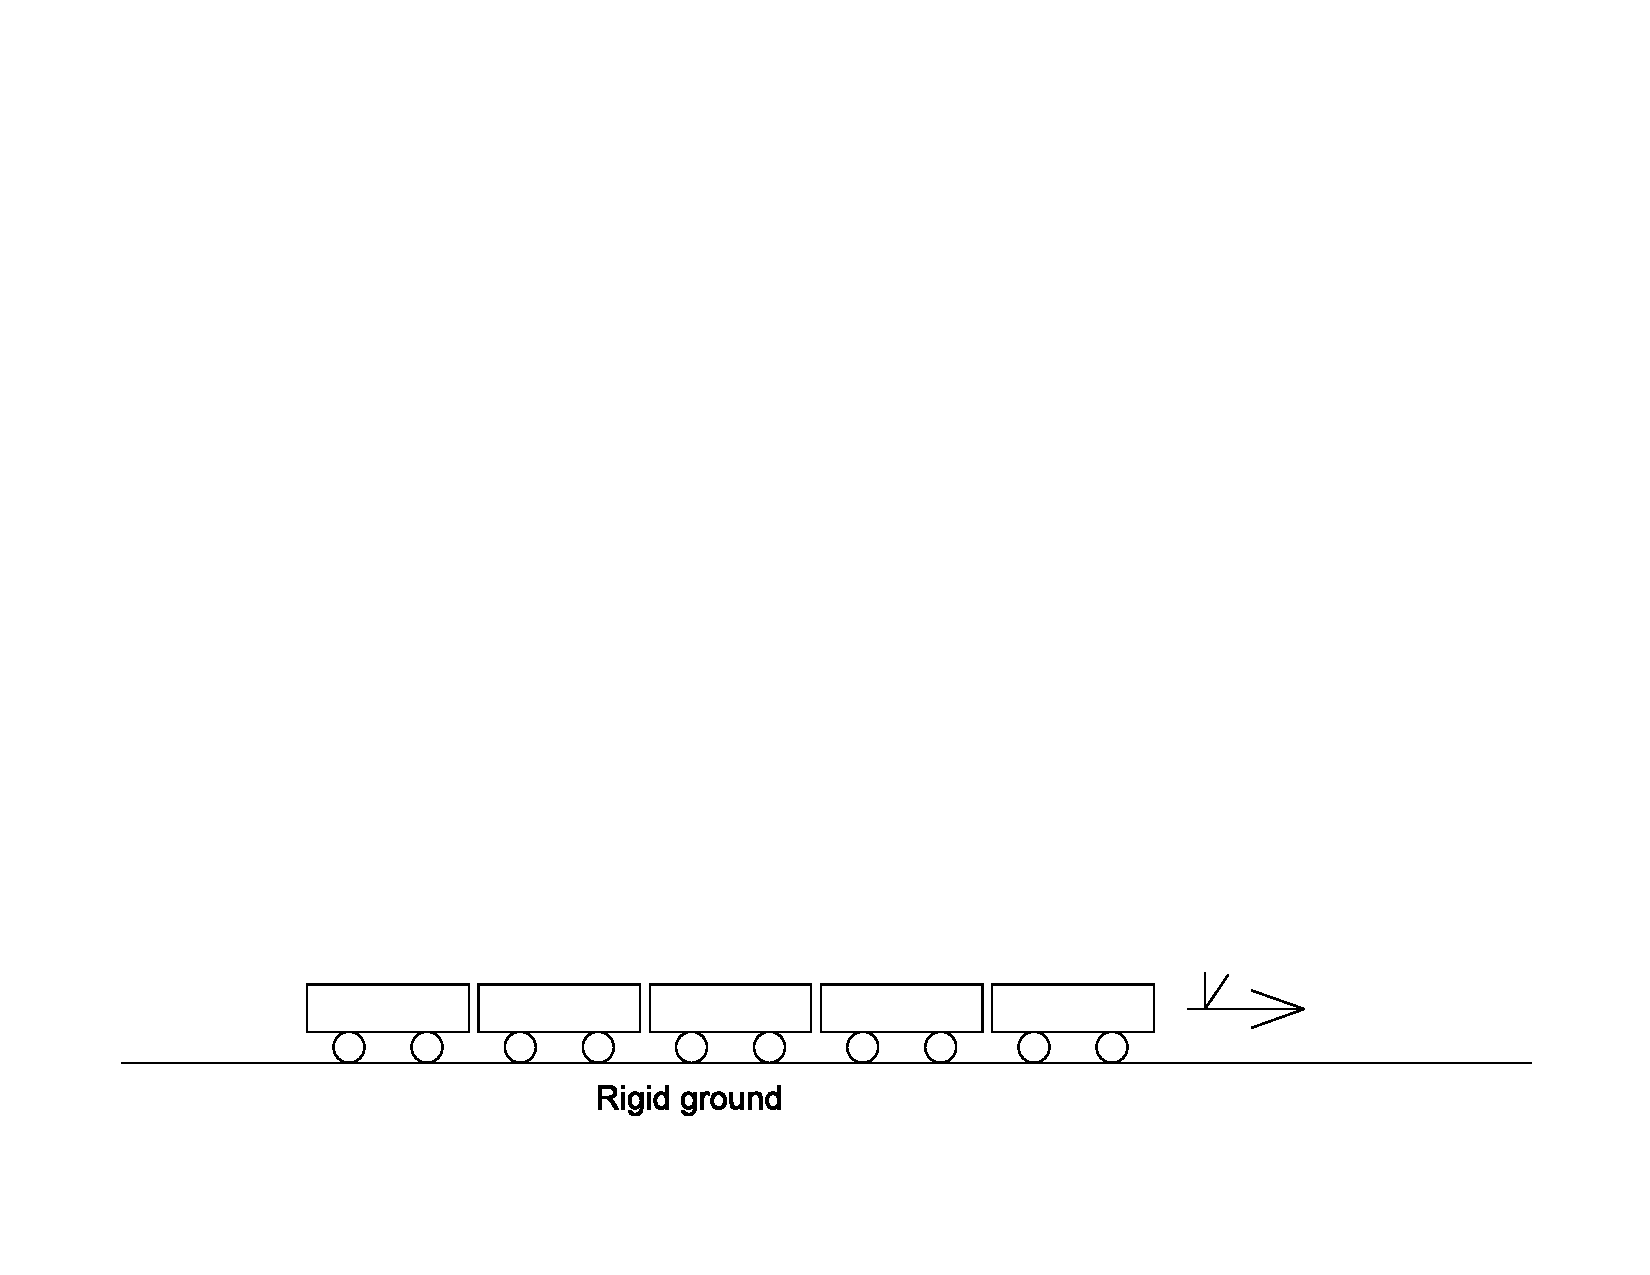
\includegraphics[width=0.8\textwidth]{trainmodellateralsimplecomplete.pdf}
%     \caption{Complete train model on rigid ground}
%     \label{fig:trainmodellateralsimplecomplete}
% \end{figure}


% \subsection{Coupled system modelling}
% From now on train model will move on bridge decks modelled as simply supported beams.

% Only one span of beam will be modelled because in RP6\cite[2.3]{d181} following statement mentioned 'there is no evidence that the resonant behaviour of the span has any effect on subsequent spans, since the resonant effects do not appear to grow from span to span.'. 

% Relative interfacing between track and bridge structure will be neglected. Thus ballast will not be modelled. Track and bridge structure will be modelled as a whole to shorten calculation time. 

% The interfacing of two systems will be investigated by following parametric studies.

% Till this step the basics of modelling are finished. Future parametric studies will use this 

% \begin{figure}[h]
%     \centering
%     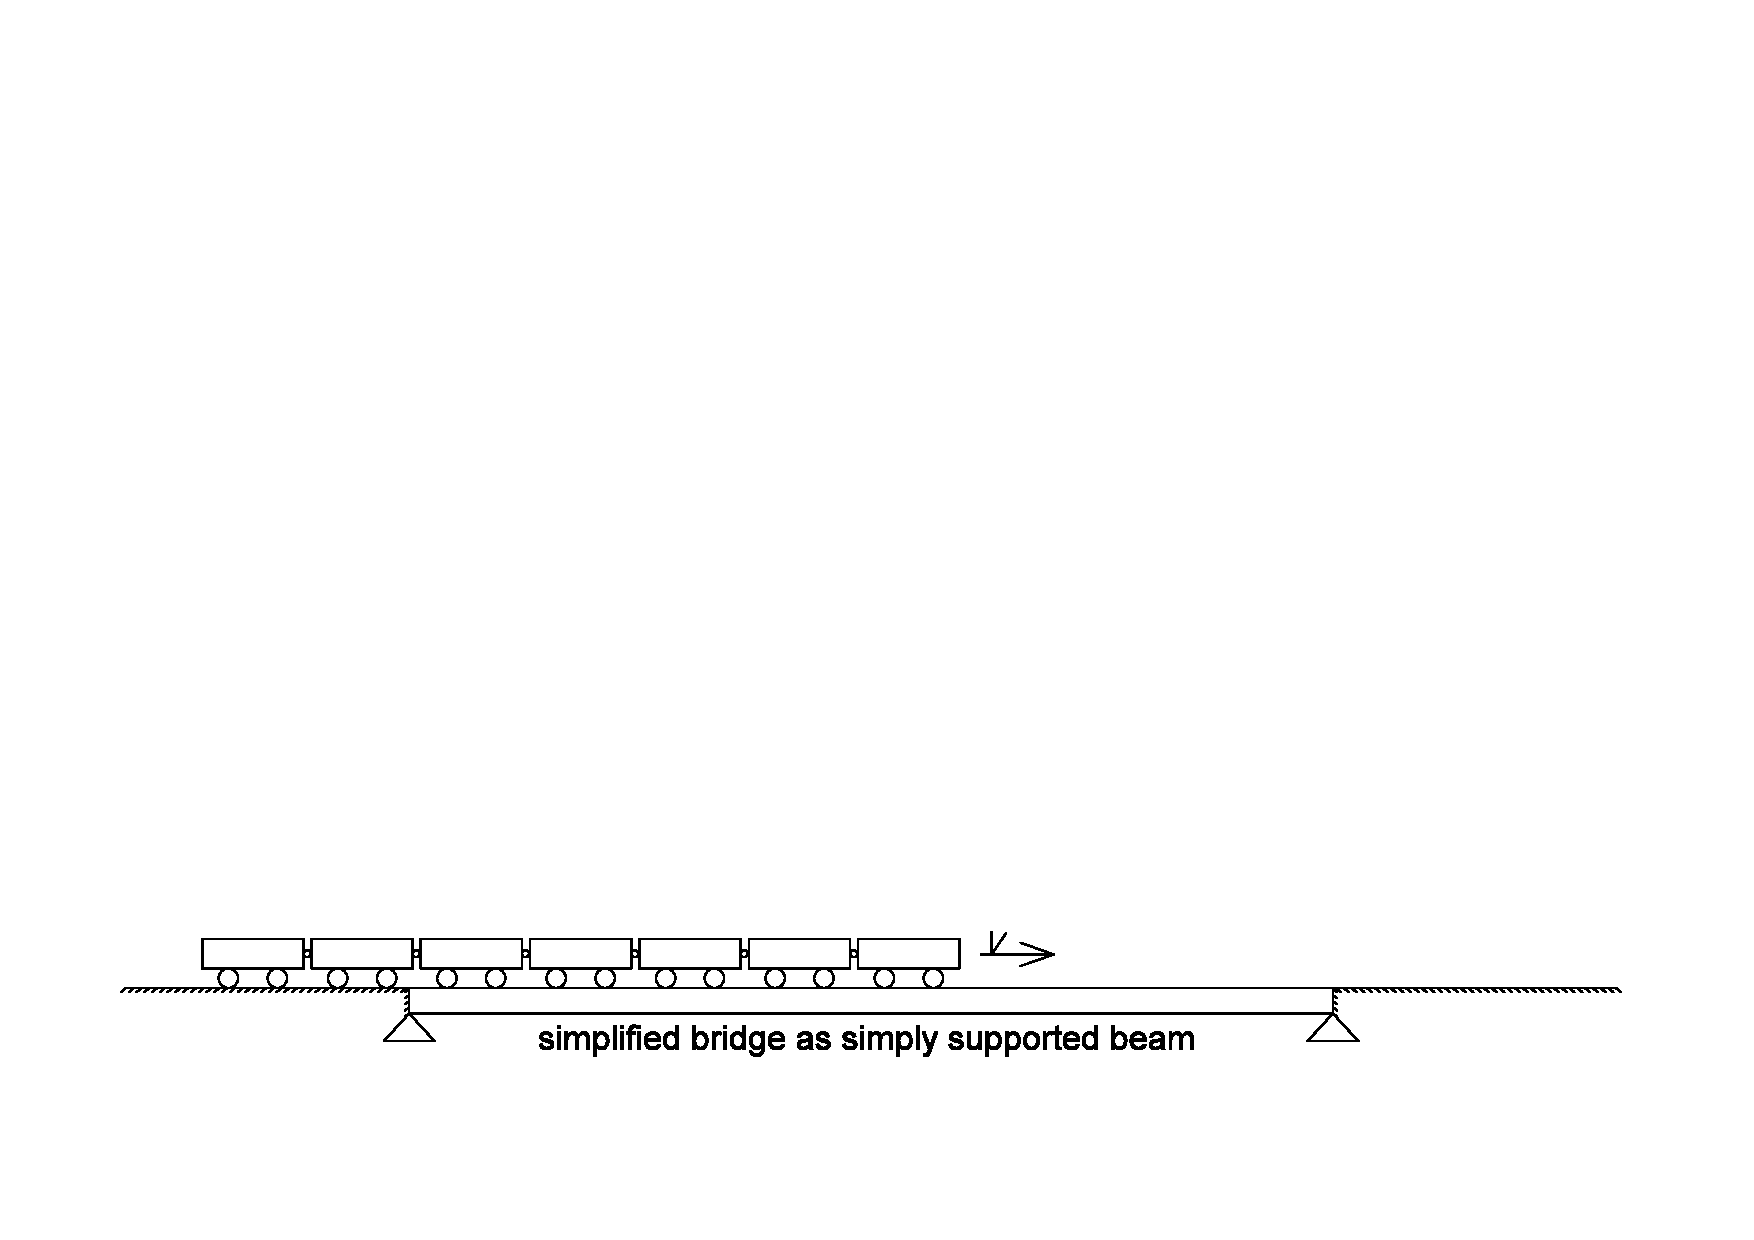
\includegraphics[width=0.8\textwidth]{trainmodellateral.pdf}
%     \caption{View of vehicle-Structure coupling model used in FEM software from the side3}
%     \label{fig:trainmodellateral}
% \end{figure}

% Parameters to be examined:
% \begin{enumerate}
% \item different layouts
% \item suspension system stiffness
% \item mass of the train
% \item track irregularities
% \item bridge span
% \item bridge mass
% \item bridge stiffness
% \end{enumerate}

\section{Effects investigated in Parametric Study}

Effects investigated in this report will be the same effects investigated in DT 329, which is described in Sec.\ref{sec:resonanceinvestigated}. However, according to the statement in Sec.2.3[Summary of results] in the same report,

\begin{quote}
Even when the axle repeat frequency matches the first lateral bending mode of each span, there is no evidence that the resonant behaviour of the span and train has any effect on subsequent spans, since the resonant effects do not appear to grow from span to span.
\end{quote}

the third investigated resonance effect 'coincidence between the length of the span and the kinematic wavelength of the trailing vehicles' is neglected in this thesis. 


\section{Speed range of dynamic consideration}

The thesis will focus on normal speed trains because IV-Groep is only interested in normal speed train lines, which its projects are being built for. Higher boundary is set according to maximum speed allowed on Dutch railways, while lower boundary is set according to an estimation. The reason for a lower boundary speed is that dynamics issues for railway infrastructures increase with respect to vehicle speed, which means generally less concern is needed when the speed of train is low. It's certain that there exists a threshold of speed for every type of train that dynamic behaviour of them start to be a problem to concern but this threshold of speed varies from different scenarios. Till now no solid research can give a value to this threshold of speed so this is why estimation of lowest speed is adopted. 

My assumption of lower boundary of speed for consideration is 120 km/h. This is still very conservative because according to logic diagram Eurocode 1991-2\cite{EC12}, dynamic check is always needed when $V \geq 200km/h$ for vertical direction. Under same speed, the kinematic energy passed to bridge by running vehicle in vertical direction is apparently higher than that in lateral direction on a straight track. So it is believed that in lateral direction, the threshold will be even higher that 200 km/h according to Eurocode 1991-2. Value 120 km/h is taken according to \cite[Appendix F]{EC15528}: \textit{Speeds which do not require dynamic compatibility checks} where 120 km/h is the lowest speed can be found in the table, excluding special vehicle. This table is attached in this thesis in Appendix.\ref{app:speedsafe}.

Upper boundary for consideration:

Normal trains running on Dutch railway has a speed limit of 160 km/h so the upper boundary for speed is set to 160 km/h, which is also 44.44 m/s. 

$$ V_{max} = 44.44m/s $$

Lower boundary for consideration:

$$ V_{min} = 33.33m/s $$

However, it is strongly advised that future research investigate the lowest speed threshold for dynamic for consideration for train vehicles in the Netherlands due to the fact that the lower boundary used in this thesis in an assumption.

\section{Equivalent conicity used in this study}
According to \cite[Section.2.6]{esveld2001modern}, 

\begin{quote}
    Practical research has shown that over a period of time wheel profiles stabilise with wear at an equivalent conicity of 0.2 to 0.3. With regards to running stability, the equivalent conicity must remain below 0.4 and to ensure the centering effect it must be greater than 0.1.
\end{quote}

conicity range will be 0.2 to 0.3.

It is suggested that vehicle maintenance sector ensure wheels of train wheels stay in the safe zone of conicity. 


\section{Parametric Study on Frequency of Klingel movement}

Klingel movement is proposed by Klingel which can well predict the moving trend of a single wheelset on a straight railway track. However, the kinematic movement of a certain wheelset assembled into a running train is different from the movement of a single free wheelset. This is due to multiple bodies interact with each other, introducing more complicated mechanism in wheel/rail interaction. 

This parametric study focuses on Klingel movement of a single wheelset. First part of the parametric study will try to discuss the relationship of Kiingle frequency of a wheelset and kinematic movement frequency of a whole train. Second part of the parametric study will use realistic data of Dutch railway/vehilces to assess the frequency bandwidth of Dutch native trains.

Parametric to be studied:

Speed of train, radius of the wheel and conicity of the wheel. 

Gauge distance is fixed to 1435mm according to UIC standard. 

Frequency is linear to speed if other parameters are fixed.

\section{Comparison between Klingle movement and train kinematic movement studied in D181 DT329}

By comparing the result from above parametric study and kinematic wavelength obtained by D181, presented as table.C2 in original report, parametric study results show close prediction for kinematic wavelength of freight train locomotive/coach/wagon. It's because freight train suspension system is simpler and stiffer compared to passenger train's, making the behaviour of train acts more similar to the behaviour of a single wheelset of bigger mass. However, results of  wavelength of single wheelset is 33\% shorter than kinematic wavelength of train because suspension system of passenger coaches are much more sophisticated. The wavelength of passenger coach is highly related to the characteristics of its suspension systems. These data is often difficult to obtain. 



The train parameter used in this part of parametric study is attached in the Appendix.\ref{app:mu}. 

% Table generated by Excel2LaTeX from sheet 'Sheet 1'
\begin{table}[htbp]
  \centering
  \caption{Add caption}
    \begin{tabular}{rrrrrrrrr}
    \toprule
    \textbf{} & \textbf{Speed} & \textbf{Gauge} & \textbf{Base wheel distance} & \textbf{Radius} & \textbf{Conicity} & \textbf{Wavelength\_0()} & \textbf{Wavelength} & \textbf{Frequency for 1m/s} \\
    \midrule
    \textbf{BR CLASS 56 LOCOMOTIVE} & 1.0000 & 1435.0000 & 1500.0000 & 290.0000 & 0.0500 & 12.8175 & 18.5418 & 0.054 \\
    \textbf{FS E444 LOCOMOTIVE} & 1.0000 & 1435.0000 & 1500.0000 & 550.0000 & 0.0500 & 17.6517 & 25.5349 & 0.039 \\
    \textbf{FS ETR500 LOCOMOTIVE} & 1.0000 & 1435.0000 & 1500.0000 & 550.0000 & 0.0500 & 17.6517 & 25.5349 & 0.039 \\
    \textbf{UIC FREIGHT WAGON (LADEN)} & 1.0000 & 1435.0000 & 1500.0000 & 460.0000 & 0.0500 & 16.1430 & 23.3524 & 0.043 \\
    \textbf{FS ETR500 COACH} & 1.0000 & 1435.0000 & 1500.0000 & 440.0000 & 0.0500 & 15.7882 & 22.8391 & 0.044 \\
    \textbf{UIC COACH} & 1.0000 & 1435.0000 & 1500.0000 & 445.0000 & 0.0500 & 15.8776 & 22.9685 & 0.044 \\
    \textbf{} &       &       &       &       &       &       &       &  \\
    \textbf{} & 1.0000 & 1435.0000 & 1500.0000 & 500.0000 & 0.0250 & 23.8016 & 34.4313 & 0.029 \\
    \textbf{} & 1.0000 & 1435.0000 & 1500.0000 & 500.0000 & 0.2000 & 8.4151 & 12.1733 & 0.082 \\
    \textbf{} & 1.0000 & 1435.0000 & 1500.0000 & 500.0000 & 0.3000 & 6.8709 & 9.9395 & 0.101 \\
    \textbf{} &       &       &       &       &       &       &       &  \\
    \textbf{} & 1.0000 & 1435.0000 & 1500.0000 & 460.0000 & 0.0250 & 22.8297 & 33.0253 & 0.030 \\
    \textbf{} & 1.0000 & 1435.0000 & 1500.0000 & 460.0000 & 0.2000 & 8.0715 & 11.6762 & 0.086 \\
    \textbf{} & 1.0000 & 1435.0000 & 1500.0000 & 460.0000 & 0.3000 & 6.5904 & 9.5336 & 0.105 \\
    \bottomrule
    \end{tabular}%
  \label{tab:addlabel}%
\end{table}%




\section{Assess of frequency bandwidth based on realistic data of Dutch Rail/Vehicle}

The wavelength of passenger coach is highly related to the characteristics of its suspension systems. These data is often difficult to obtain. To establish an easy approach, wavelength of passenger train calculated in this section will be multiplied by an amplification factor of 1.5. This value is obtain by train wavelength/wheelset wavelength ratio in previous parametric study. Please note this factor is an estimation. However, wavelength of freight train is not modified due to the conclusion that freight train's suspension system is stiff enough for the Klingle movement of a single wheelset to describe the kinematic movement of a whole freight train.

However, future research is highly recommended to be conducted to study the kinematic wavelength of complete vehicles in the Netherlands, using realistic data of their suspension systems.

Klingel's formula:
Klingel has done experiments and has given that the wavelength of a single wheelset:

$$ \lambda_0 = 2 \pi \sqrt{\frac{rG}{2\gamma} }$$

where:

G = Dynamic Gauge

r = Dynamic Wheels Radius

g = Conicity

For 2 wheelsets connected by a bogie:

$$ \lambda = \lambda_0 \sqrt{1+(\frac{I}{G})^2}  $$

where:

I = Rigid wheel base

Thus range of $\lambda$ is obtained by inputing data discussed in previous sections of this chapter.

Following plots are generated according to linear relationship between frequency and speed:

$$ f = v \frac{1}{\lambda} $$


\begin{figure}[h!]
\centering
\begin{tikzpicture}[trim axis left, trim axis right]
\begin{axis}[
    title = {Lateral frequency of freight train with respect to speed},
    xlabel={$v(m/s)$},
    ylabel={$f(Hz)$},
    ymin = 0, xmin = 0, xmax = 44.4,
    legend entries={$\sfrac{1}{\lambda}=0.059$,$\sfrac{1}{\lambda} =0.072$,$v=33.3 m/s$,$f=0.3Hz$},
    grid = both,
    minor y tick num= 4,
    minor x tick num= 4,
    legend pos = north west,
]
\addplot[blue, domain = 0:44.4,samples=201,name path = A]{0.059*x};
\addplot[red, domain = 0:44.4,samples=201, name path = B]{0.072*x};
\addplot[mark=none, dashed]  coordinates {(33.3,0) (33.3,5) };
\addplot[domain = 0:44.4,samples=10,dashed]{0.3};
\addplot[gray] fill between[of=A and B];
\end{axis}
\end{tikzpicture}
\end{figure}

\begin{figure}[h!]
\centering
\begin{tikzpicture}[trim axis left, trim axis right]
\begin{axis}[
    title = {Lateral frequency of passenger train with respect to speed},
    xlabel={$v(m/s)$},
    ylabel={$f(Hz)$},
    ymin = 0, xmin = 0, xmax = 44.4,
    legend entries={$\sfrac{1}{\lambda}=0.062$,$\sfrac{1}{\lambda}=0.076$,$v=33.3 m/s$,$f=0.3Hz$},
    grid = both,
    minor y tick num= 4,
    minor x tick num= 4,
    legend pos = north west,
]
\addplot[blue, domain = 0:44.4,samples=201, name path = A]{0.062*x};
\addplot[red, domain = 0:44.4,samples=201, name path = B]{0.076*x};
\addplot[mark=none,dashed]  coordinates {(33.3,0) (33.3,3.5) };
\addplot[domain = 0:44.4,samples=10,dashed]{0.3};
\addplot[gray] fill between[of=A and B];
\end{axis}
\end{tikzpicture}

\end{figure}

\section{Parametric study on frequency caused by axle repeat pattern}

Following wavelength of axle repeat pattern is obtained by extracting MU standards in \cite{EC15528}. Detailed information can be found in Appendix.\ref{app:mu}
% Table generated by Excel2LaTeX from sheet 'Axle repeat pattern'
\begin{table}[h!]
  \centering
  \caption{Wavelength of axle repeat pattern(m)}
    \begin{tabular}{rrrrrrrrr}
    \toprule
    \textbf{Type} & \textbf{L\_coa min} & \textbf{L\_coa max} & \textbf{2*L\_coa min } & \textbf{2*L\_coa max} \\
    \midrule
    \textbf{CB\_1} & 23.8  & 25.3  & 47.6  & 50.6 \\
    \textbf{CB\_2} & 25.3  & 27.5  & 50.6  & 55    \\
    \textbf{AB\_1} & 14.9  & 16    & 29.8  & 32     \\
    \textbf{AB\_2} & 18.8  & 19.5  & 37.6  & 39    \\
    \textbf{AB\_3} & 17    & 17.5  & 34    & 35   \\
    \textbf{AB\_4} & 18.7  & 19.2  & 37.4  & 38.4  \\
    \textbf{SA\_1} & 9.2   & 9.8   & 18.4  & 19.6  \\
    \textbf{SA\_2} & 12.8  & 13.5  & 25.6  & 27    \\
    \bottomrule
    \end{tabular}%
  \label{tab:wavelengthaxlerepeat}%
\end{table}%

Range of wavelength(m) of first repeat pattern mode:

$$ \lambda_{1stRepeat} \in (9.2,9.8) \cup (12.8,13.5) \cup (14.9, 16) \cup (17,17,5) \cup (18.7, 19.5) \cup (23.8,27.5)$$

Range of wavelength(m) of second repeat pattern mode:

$$ \lambda_{2ndRepeat} \in (18.4,19.6) \cup (25.6,27) \cup (29.8, 32) \cup (34,35) \cup (37.4, 39) \cup (37.6,55)$$

Range of frequency(Hz) yielded by dividing 1m/s with wavelength of first repeat pattern mode:

$$ \frac{1}{\lambda_{1stRepeat}} \in (0.036,0.042) \cup (0.051,0.053) \cup (0.057,0.059) \cup (0.063,0.067) \cup (0.074,0.078) \cup (0.102,0.109)   $$

Range of frequency(Hz) yielded by dividing 1m/s with wavelength of second repeat pattern mode:

$$ \frac{1}{\lambda_{2ndRepeat}} \in (0.018,0.021) \cup (0.026,0.027) \cup (0.029,0.029) \cup (0.031,0.034) \cup (0.037,0.039) \cup (0.051,0.054)   $$

Following plot is generated according to linear relationship between frequency and speed:

$$ f = v \frac{1}{\lambda_{repeat}} $$

\begin{figure}[h]
\centering
\begin{tikzpicture} 
    \begin{axis}[
    title = {Two repeat pattern frequencies with respect to speed},
    xlabel={$v(m/s)$},
    ylabel={$f(Hz)$},
    ymin = 0, xmin = 0, xmax = 44.4,
    %legend entries={$i=0.057$,$i=0.07$,$v=33.3 m/s$,$f=0.3Hz$},
    grid = both,
    minor y tick num= 4,
    minor x tick num= 4,
    ]
    \addplot[blue,name path=A,domain=0:44.4] {0.036*x};
    \addplot[red, name path=B,domain=0:44.4] {0.042*x};
    \addplot[black] fill between[of=A and B];
    \addplot[blue,name path=C,domain=0:44.4] {0.051*x};
    \addplot[red, name path=D,domain=0:44.4] {0.053*x};
    \addplot[black] fill between[of=C and D];
    \addplot[blue,name path=E,domain=0:44.4] {0.057*x};
    \addplot[red, name path=F,domain=0:44.4] {0.059*x};
    \addplot[black] fill between[of=E and F];
    \addplot[blue,name path=G,domain=0:44.4] {0.063*x};
    \addplot[red, name path=H,domain=0:44.4] {0.067*x};
    \addplot[black] fill between[of=G and H];
    \addplot[blue,name path=I,domain=0:44.4] {0.074*x};
    \addplot[red, name path=J,domain=0:44.4] {0.078*x};
    \addplot[black] fill between[of=I and J];
    \addplot[blue,name path=K,domain=0:44.4] {0.102*x};
    \addplot[red, name path=L,domain=0:44.4] {0.109*x};
    \addplot[black] fill between[of=K and L];
    \addplot[blue,name path=M,domain=0:44.4] {0.018*x};
    \addplot[red, name path=N,domain=0:44.4] {0.021*x};
    \addplot[gray] fill between[of=M and N];
    \addplot[blue,name path=O,domain=0:44.4] {0.026*x};
    \addplot[red, name path=P,domain=0:44.4] {0.027*x};
    \addplot[gray] fill between[of=O and P];
    \addplot[blue,name path=Q,domain=0:44.4] {0.029*x};
    \addplot[red, name path=R,domain=0:44.4] {0.029*x};
    \addplot[gray] fill between[of=Q and R];
    \addplot[blue,name path=S,domain=0:44.4] {0.031*x};
    \addplot[red, name path=T,domain=0:44.4] {0.034*x};
    \addplot[gray] fill between[of=S and T];
    \addplot[blue,name path=U,domain=0:44.4] {0.037*x};
    \addplot[red, name path=V,domain=0:44.4] {0.039*x};
    \addplot[gray] fill between[of=U and V];
    \addplot[blue,name path=W,domain=0:44.4] {0.051*x};
    \addplot[red, name path=X,domain=0:44.4] {0.054*x};
    \addplot[gray] fill between[of=W and X];
    \addplot[dashed,thick,red, domain=0:44.4] {0.3};
\end{axis}
\end{tikzpicture}
\end{figure}

\section{Conclusion of parametric study}

This parametric study illustrates a tool of obtaining danger zone for train speed for a specific bridge first lateral natural frequency. 

For example, if a bridge has a first lateral natural frequency of 0.3Hz:

\begin{enumerate}
\item To avoid resonance between freight train and bridge caused by kinematic frequency coincidence, speed of train should be regulated above 4m/s

\item To avoid resonance between passenger train and bridge caused by kinematic frequency coincidence, speed of train should be regulated above 5m/s

\item To avoid resonance caused by axle repeat pattern, speed of train should be regulated above 16m/s

\end{enumerate}

As a conclusion, if the speed of train is regulated above 16m/s, there won't be resonance between bridge and train.

\chapter{Recommendations on improvement on Eurocode}


\section{Another criterion proposed by J.J.Reber}
A SNCB bridge, driver complains 

To be used in combination with Sijian Deng's criterion.

\section{Misc}

Define eigen frequency and natural frequency

Define how-to-do and what-to-do a dynamic analysis

\section{Improve criteria for lateral bridge dynamics}
Following sections provides several orientations for improving criteria for lateral bridge dynamics in terms of safety and serviceability of running stock.


\subsection{Requirements for traffic safety(horizontal)}
Requirements other than bridge first lateral frequency higher than 1.2Hz. Since there's no further requirements mentioned by Eurocode, following requirements are gathered from other European codes, eg. British standards, UIC leaflet, etc.

\begin{enumerate}[-]
    \item Requirements regarding traffic safety for vehicles
    \begin{enumerate}
        \item Guiding Force: \cite{code2005518} , \cite{en200714363} and\cite{cuadrado2008analysis} propose safty limitations against railway vehicle overturning. From\cite{en200714363} the maximum guiding force for a vehicle with a load per axle of 170kN(AVE) is 66kN per axle and 48kN per axle for a vehicle with a load per axle of 112kN(ICE2). For the R1 freight wagon(load per axle of 245kN), the maximum guiding force per axle is 78kN.
        \item Maximum lateral acceleration of the railway vehicle: proposed by \cite{13803}
    \end{enumerate}
    \item Requirements regarding safety for bridge\\
    \cite{EC0} A2.4.4.1(2): Horizontal transverse deflection(to ensure acceptable horizontal track radii) and horizontal rotation of a deck about a vertical axis at ends of a deck(to ensure acceptable acceptable horizontal track geometry and passenger comfort)
\end{enumerate}


\subsection{Requirements for traffic safety on derailment: Railway vehicle derailment mechanism and safety criteria}

Derailment mechanisms
\begin{enumerate}
    \item vehicle resonant response
    \item lateral instability
    \item vehicle overturning
    \item vertical wheel unloading
    \item flange climb
    \item rail roll-over
    \item track panel shift
    \item longitudinal train forces
\end{enumerate}

The four types of derailment: flange climb derailment, derailment caused by guage widening and rail roll-over, derailment caused by track panel shift, derailment cause by vehicle lateral instability have a common cause of high lateral force at the wheel-rail interface. According to \cite[Chapter 8, IV]{iwnicki2006handbook} any conditions that lead to high lateral forces or lead to lower the ability of the system to sustain the force should be corrected. 

\subsubsection{Flange climb derailment}
Wheel flange climb derailments are caused by wheels climbing onto the top of the railhead then further running over the rail. Wheel climb derailments generally occur in situations where the wheel experiences a high lateral force combined with circumstances where the vertical force is reduced on the flanging wheel. The high lateral force is usually induced by a large wheelset angle-of-attack. The vertical force on the flanging wheel can be reduced significantly on bogies having poor vertical wheel load equalisations, such as when negotiating rough track, large track twist, or when the car is experiencing roll resonances. 

\begin{figure}[h]
    \centering
    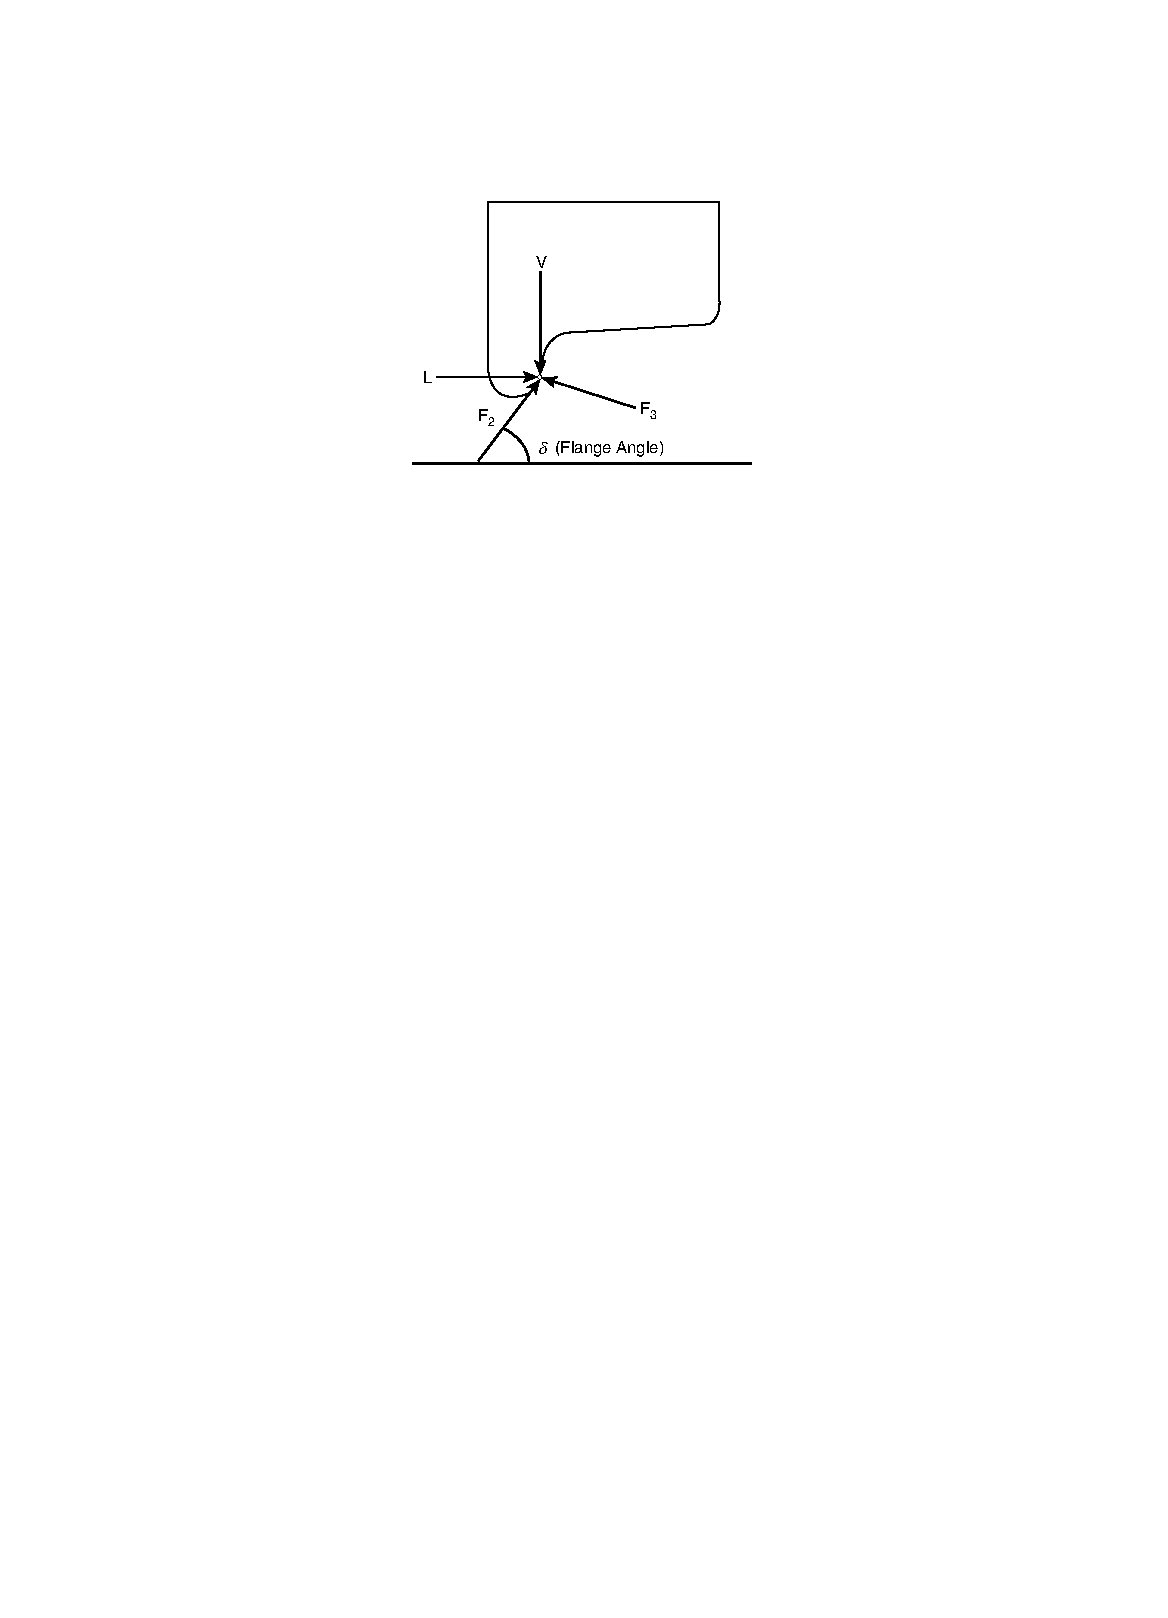
\includegraphics[width=0.4\textwidth]{forcesatflangecontactlocation.pdf}
    \caption{Forces at flange contact location. Extracted from \cite[Figure8.4]{iwnicki2006handbook}}
    \label{fig:forcesatflangecontactlocation}
\end{figure}

The criterion L/V ratio can be expressed as:

\begin{equation}
    \frac{L}{V}=\frac{\tan \delta -\frac{F_2}{F_3}}{1+\frac{F_2}{F_3}\tan \delta}
\end{equation}

Nadal's famous L/V ratio limiting criterion, given by Equation.\ref{eq:nadalcriterion}, was proposed for the saturated condition $F_2/F_3=\mu$

\begin{equation}\label{eq:nadalcriterion}
    \frac{L}{V}=\frac{\tan \delta - \mu}{1+ \mu \tan \delta}
\end{equation}

\subsubsection{Derailment caused by guage widening and rail rollover}
Derailments caused by guage widening usually involve a combination of wide gauges and large lateral rail defections(rail roll), as shown in Figure\ref{fig:gaugewideningderailment}. Large lateral forces from the wheels act to spread the rails in curves. Both rails may experience significant lateral translation and/or railhead roll, which often cause the nonflanging wheel to drop between rails.

\begin{figure}[h]
    \centering
    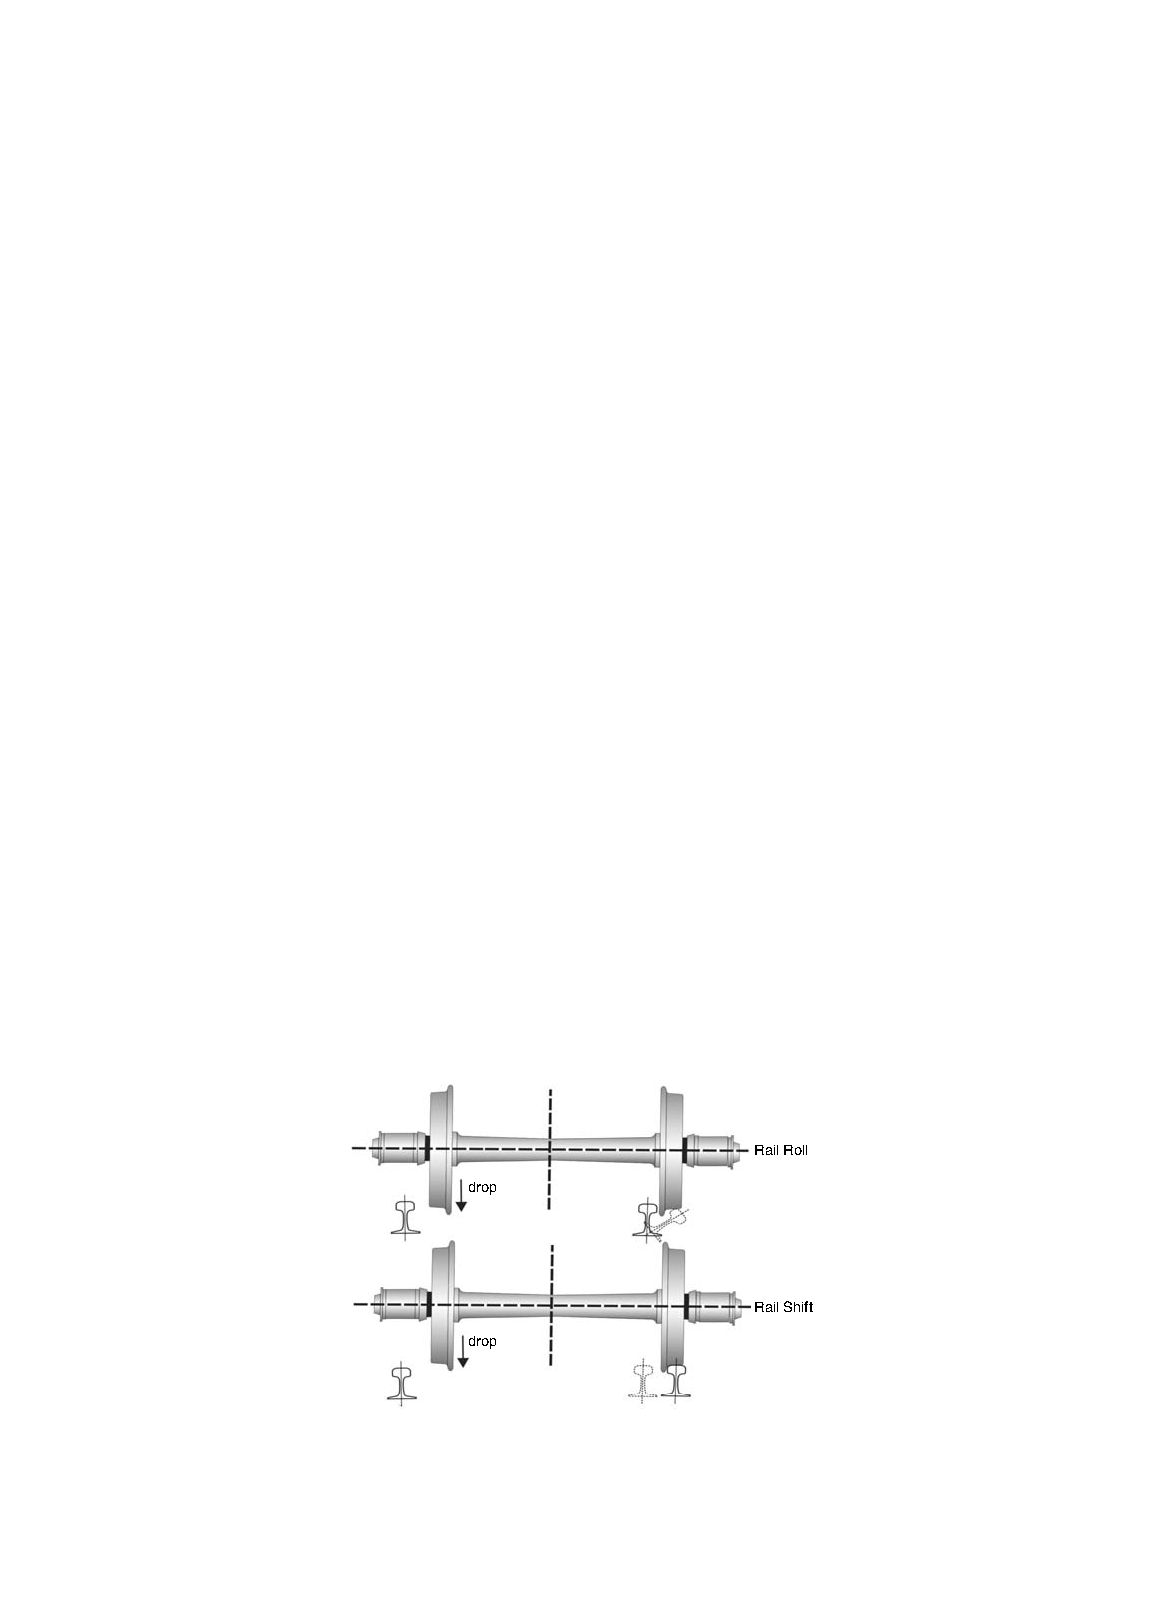
\includegraphics[width=0.8\textwidth]{gaugewideningderailment.pdf}
    \caption{Gauge widening derailment. Extracted from \cite[Figure8.18]{iwnicki2006handbook}}
    \label{fig:gaugewideningderailment}
\end{figure}

\paragraph{AAR Chapter XI rail roll criterion}
The AAR Chapter XI rail roll criterion is established by using the L/V ratio. The roll moment about the pivot point is given by,

\begin{equation}
    M=Vd-Lh
\end{equation}

under an equilibrium condition, just before the rail starts to roll, $M$ approaches to zero, then,

\begin{equation}
    \frac{L}{V}=\frac{d}{h}
\end{equation}

This L/V ratio is considered as the critical value to evaluate the risk of rail roll. When the L/V ratio is larger than the ratio of $d/h$, the risk of rail roll becomes high. The critical L/V ratio for rail roll can vary from above 0.6 for contact at the gauge side to approximately 0.2 when the contact position is at the far-field side based on the dimension of the rails. This is because the distance $d$ is reduced. Note that this L/V ratio is calculate assuming that neither the rail fasteners nor the torsional stiffness of the rail section provide any restraint.

\subsubsection{Derailment caused by track panel shift}
Track panel shift is the cumulative lateral displacement of the track panel, including rails, tie plates and ties, over the ballast, as shown in Figure\ref{fig:lateraltrackpanelshift}. A small shift of these components may not immediately cause the loss of guidance to bogies. However, as the situation gradually depreciates to a certain level, wheels could lose guidance and drop to the ground at some speed. The derailments caused by track panel usually result in one wheel falling between the rails and the other falling outside of the track.

\begin{figure}[h]
    \centering
    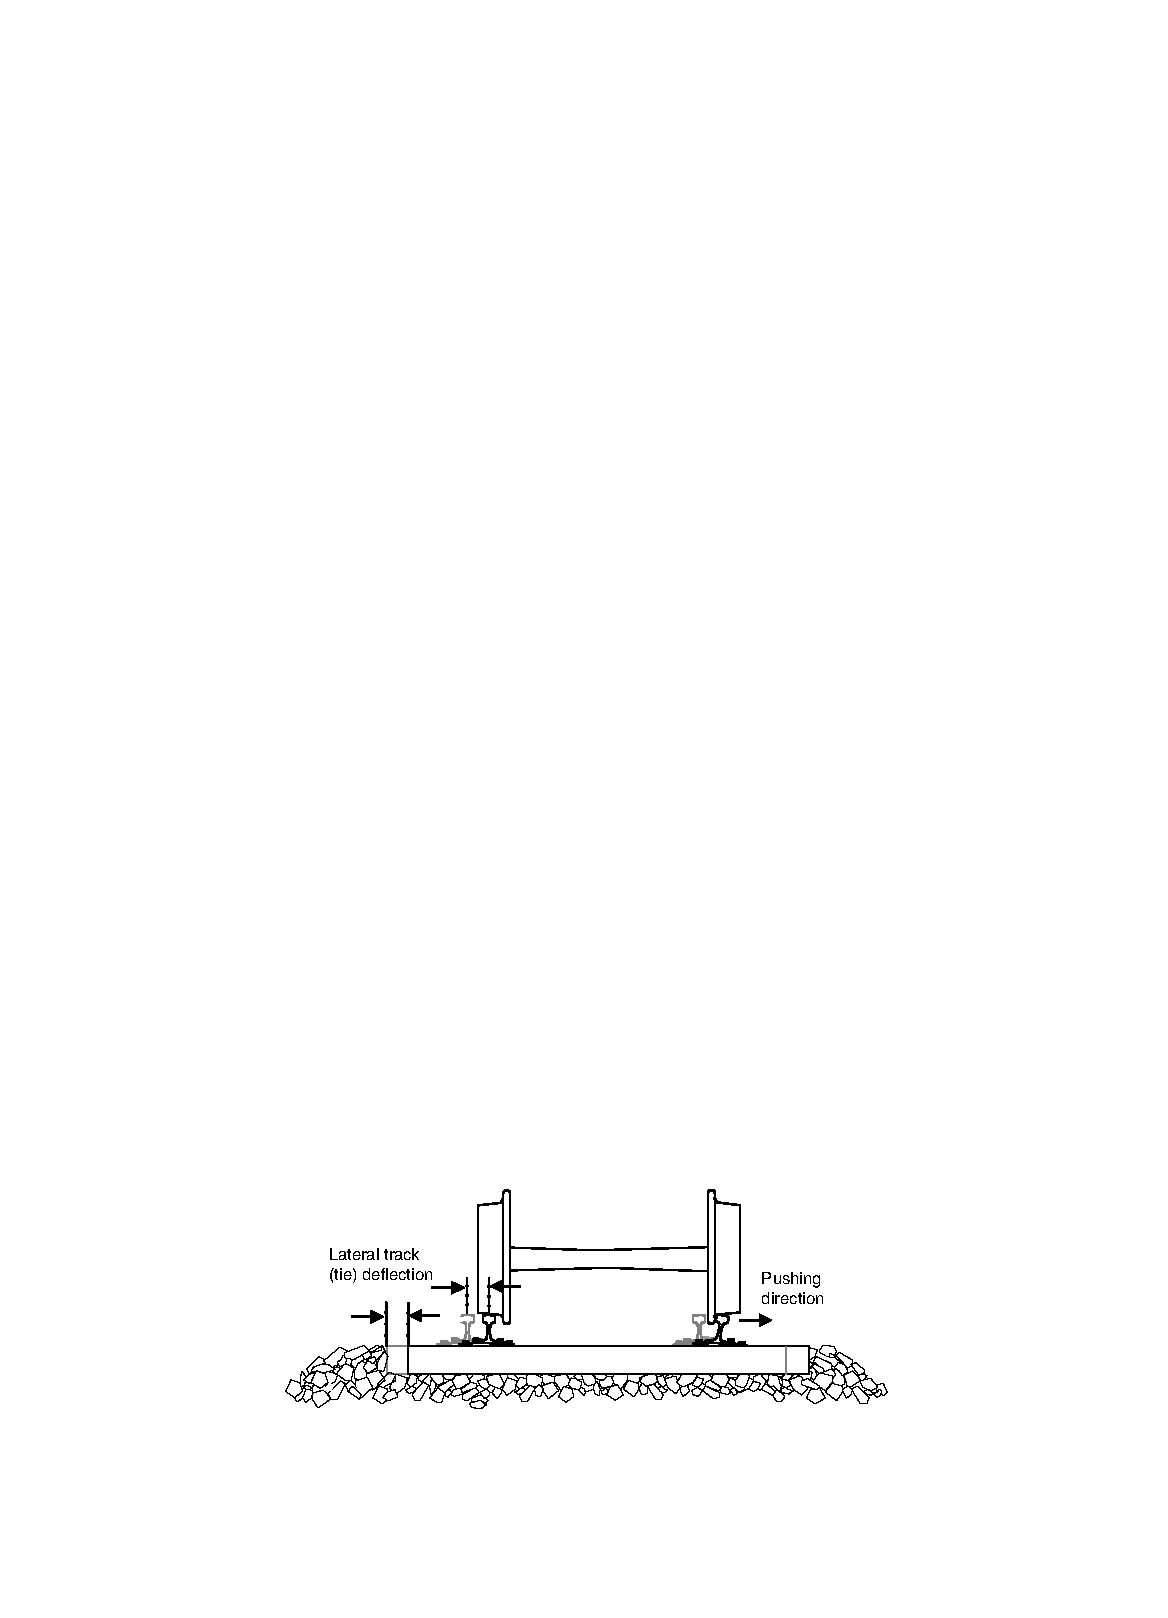
\includegraphics[width=0.8\textwidth]{lateraltrackpanelshift.pdf}
    \caption{Lateral track panel shift. Extracted from \cite[Figure8.27]{iwnicki2006handbook}}
    \label{fig:lateraltrackpanelshift}
\end{figure}

\paragraph{Panel shift criterion}
Researched by the French National Railways suggested that the limiting lateral axle load can be defined in a general expression for preventing excessive track panel shift:

\begin{equation}
    L_c = aV+b
\end{equation}

where $L_c$ is the critical lateral load and $V$ is the vertical axle load. \cite[Table 8.2]{iwnicki2006handbook} lists two groups of suggested valued of $a$ and $b$. It is possible that different values for $a$ and $b$ can be specified in different area.

\subsubsection{Derailment caused by vehicle lateral instability}
On tangent track, the wheelset generally oscillates around the track centre due to any vehicle and track irregularities, as shown in Figure\ref{fig:wheelsetoscillatesaroundthetrackcentre}. This movement occurs because vehicle and track are never absolutely smooth and symmetric. This self-centring capability of a wheelset is induced by the coned shape of the wheel tread. However, as speed is increased, if the whelset conicity is high, the lateral movement of wheelset, as well as the associated bogie and car body motion, can cause oscillations with large amplitude  and a well-defined wavelength. The lateral movements are limited only by the contact of the wheel flanges with the rail. This vehicle dynamic response is also termed as vehicle hunting, and can produce high lateral forces to damage track to cause derailments.

\begin{figure}[h]
    \centering
    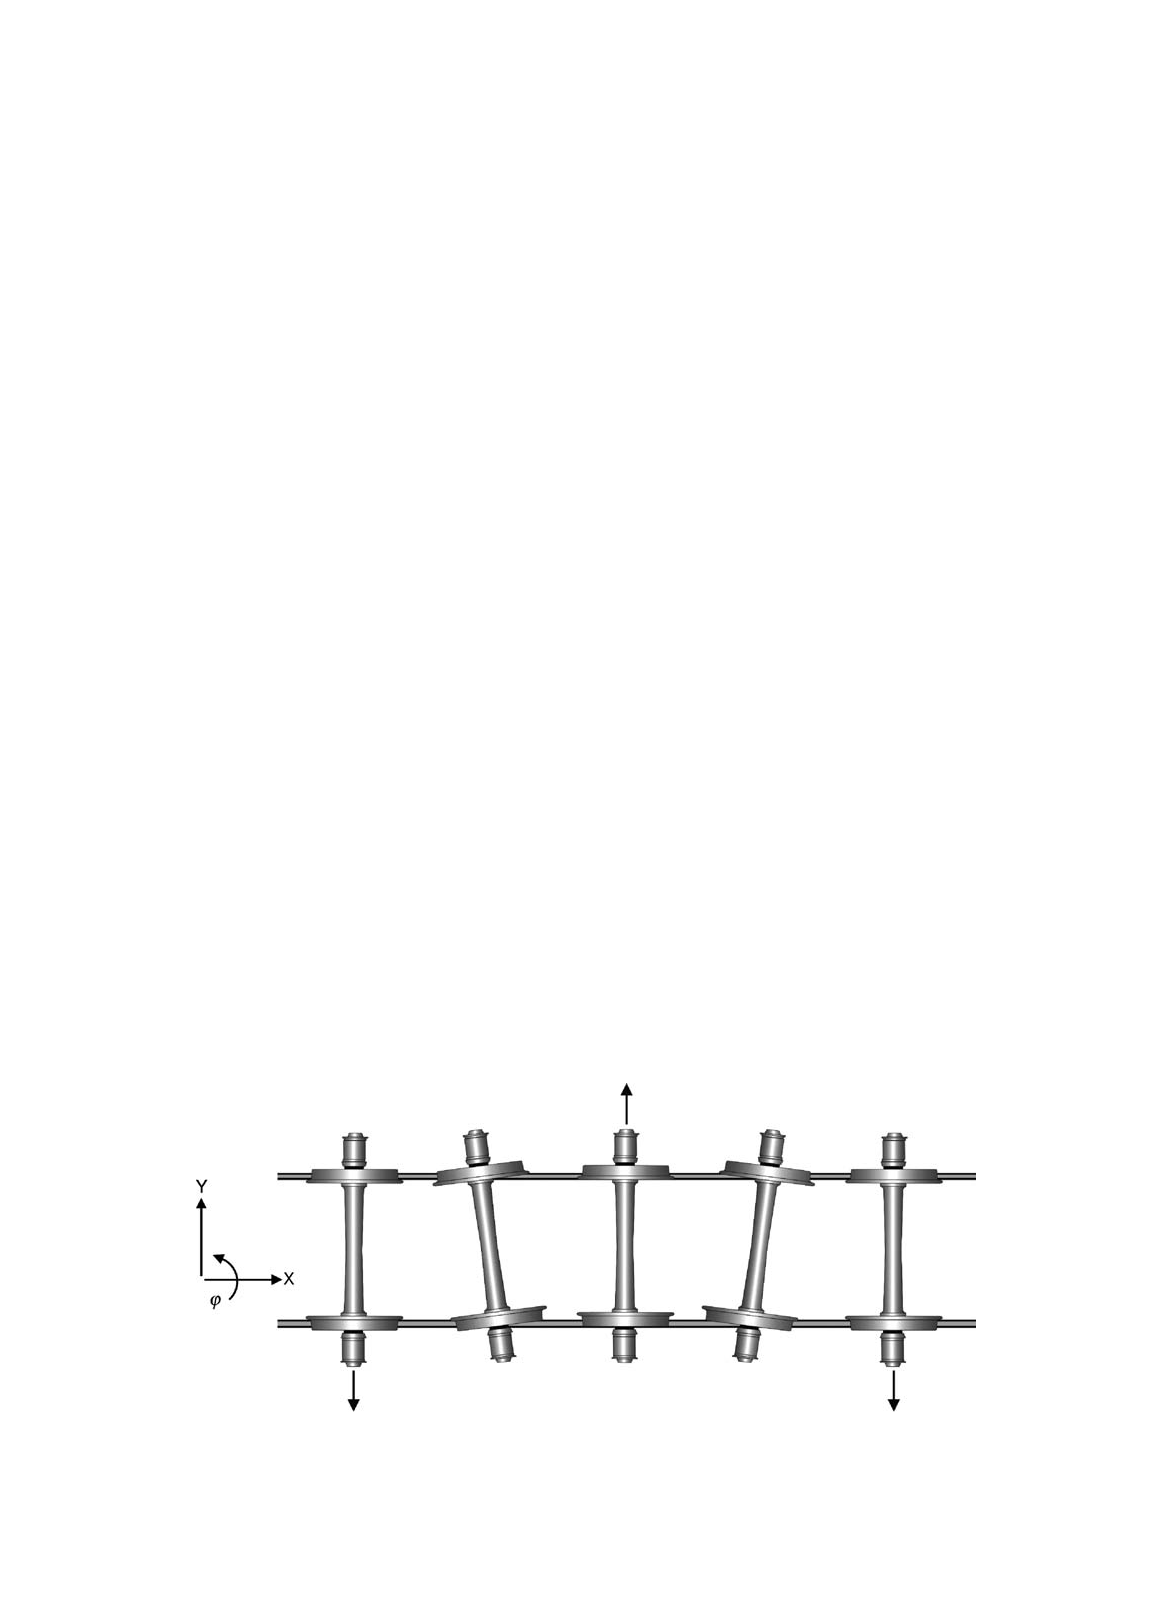
\includegraphics[width=0.8\textwidth]{wheelsetoscillatesaroundthetrackcentre.pdf}
    \caption{Wheelset oscillates around the track centre. Extracted from \cite[Figure8.28]{iwnicki2006handbook}}
    \label{fig:wheelsetoscillatesaroundthetrackcentre}
\end{figure}

Derailment cause by vehicle hunting can have derailment mechanisms of all four types discussed in the previous sections. The high lateral force induced from hunting may cause wheel flange climbing on the rail, gauge widening, rail roll-over, track panel shift, or combinations of these. The safety concerns for this type of derailment, usually occurring at higher speeds, make it an important area of study.

Hunting predominantly occurs in empty or lightweight vehicles. The critical hunting speed is highly dependent on the vehicle/track characteristics. Investigation of the critical speed for such a system with nonlinearities is to examine the vehicle response to a disturbance using a numerical solution of the equations of motion.

\subsection{Requirements for traffic serviceability(horizontal)}

The criteria Comfort Indexes for assessing ride comfort in railway vehicles proposed in \cite{12299}. This standard describes a methodology for assessing ride comfort as a function of longitudinal, vertical and transverse accelerations.

Comfort Index indicates the percentage of passengers experimenting discomfort in a specific situation. These indexes can be computed via empiric formula given in the standard, which depend on variables such as lateral acceleration, rate of change of acceleration and rolling velocity. All these values are filtered with a moving average filter that eliminates small wavelength components. Using this methodology for the computed worst-case situations, the comfort indexes have been found excellent, therefore no passenger should feel uncomfortable.
